\documentclass[a4paper,review,12pt,authoryear]{elsarticle}

% \usepackage{natbib}
\usepackage{amsfonts,amsmath,bbm,bm,xcolor,booktabs,hyperref,amsthm}
\usepackage{geometry}
\usepackage{hyperref}
\usepackage{subfig}
\geometry{a4paper,scale=0.8}
\usepackage{setspace}
\setstretch{1.5}
\let\code=\texttt
\let\proglang=\textsf
\setcounter{MaxMatrixCols}{20}
\usepackage{enumitem}


% Define a new counter for your research questions
\newcounter{researchquestion}
\setcounter{researchquestion}{0}

% Define the environment for the research questions
\newenvironment{researchquestion}{%
    \refstepcounter{researchquestion}%
    \par\medskip\noindent%
    \textbf{RQ\theresearchquestion.}~%
}{\medskip}



\hypersetup{
  colorlinks=true,
  linkcolor=blue,
  citecolor=blue,
  urlcolor=blue}

% ADDING LINENUMBERS FOR REVIEWING:
% \usepackage{lineno}

\begin{document}

\begin{frontmatter}

  %\title{On the performance of hierarchy construction: impacts of structure and clustering}
\title{Augmenting hierarchical time series through clustering: \\Is there an optimal way for forecasting?}



  \author[label1]{Bohan Zhang\corref{cor1}}
  \address[label1]{School of Economics and Management, Beihang University, Beijing, China}
  \ead{zhangbohan@buaa.edu.cn}
  \cortext[cor1]{Corresponding author.}
  \author[label2]{Anastasios Panagiotelis}
  \address[label2]{The University of Sydney Business School, NSW 2006, Australia}
  \author[label3]{Han Li}
  \address[label3]{Department of Economics, The University of Melbourne, VIC 3010, Australia}

  \begin{abstract}

    Forecast reconciliation has attracted significant research interest in recent years, with most studies relying on pre-defined hierarchies constructed with time series metadata. With the goal of improving forecast accuracy in mind, we extend and contribute to the emerging research on the clustering-based reconciliation method by proposing a novel framework for hierarchy construction. This framework offers three approaches: cluster hierarchies, random hierarchies, and combination hierarchies. Utilizing the proposed approaches, we investigate the individual contributions of two primary factors, namely ``grouping'' and ``structure'', to the performance of forecast reconciliation.  Through a simulation study and experiments on two real-world datasets, we demonstrate the practical efficacy of different hierarchy construction approaches. Our findings provide new insights into the dynamics between ``grouping'' and ``structure'', which lead to an improved understanding of forecast reconciliation.\\

  \end{abstract}

  \begin{keyword}
  Forecast reconciliation \sep
  Hierarchical time series \sep
  Clustering \sep
  Hierarchy construction \sep
  Forecast combination
  \end{keyword}

\end{frontmatter}

%\clearpage
\newpage
% \linenumbers

\section{Introduction}

Applications where some variables are aggregates of one another, or so-called \textit{hierarchical time series (HTS)}, are found in many forecasting problems ranging from supply chain management (\citealp{syntetosSupplyChainForecasting2016}) to tourism planning (\citealp{kourentzesCrosstemporalCoherentForecasts2019}), electrical load forecasting (\citealp{jeonProbabilisticForecastReconciliation2019}), and retail demand forecasting (\citealp{makridakisM5AccuracyCompetition2022}). In recent decades, there has been an increasing interest in hierarchical forecasting, primarily driven by the success of the optimal reconciliation framework (\citealp{hyndmanOptimalCombinationForecasts2011,wickramasuriyaOptimalForecastReconciliation2019, panagiotelisProbabilisticForecastReconciliation2023}). The original motivation for forecast reconciliation was to ensure forecasts are \textit{coherent}, that is they respect the aggregation constraints implied by the hierarchical structure. Coherent forecasts faciliate aligned decisions by agents acting upon different variables within the hierarchy. For example, consider a retail setting, where a warehouse manager supplies stock to individual store managers within their region. Forecasts could be incoherent when the warehouse manager forecasts low total demand while store managers forecast high demand, leading to supply shortages. Numerous case studies in the literature demonstrate that reconciliation approaches not only yield coherent forecasts but also enhance overall forecast performance (\citealp{AthanasopoulosForecastReconciliationReview2023}).

%The primary objective of hierarchical forecasting is to produce coherent forecasts for the series within a given HTS, which we refer to as \textit{original hierarchy}, ensuring that decision-makers at different levels of the hierarchy can analyze and make informed decisions based on aligned expectations for the future.
A limitation in the overwhelming majority of the forecast reconciliation studies is that the structure of the hierarchy is taken as \textit{given}. This structure usually includes \textit{bottom level series}, an overall aggregate or \textit{top level series}, with various aggregation schemes used to construct \textit{middle levels series}. Typically, middle levels are formed according to inherent attributes of the bottom-level series, such as geographical location, gender, product category, travel purpose, and others. We refer to this type of structure as the \textit{natural hierarchy}. While in some forecasting applications, decisions must be made with respect to the natural hierarchy, in other settings there might be some flexibility in determining how bottom levels are aggregated into middle levels. It should be noted that,  very little attention has been paid to whether middle level series can be constructed in a way that leads to further improvements in forecast accuracy relative to a given natural hierarchy. To the best of our knowledge, only \cite{pangHierarchicalElectricityTime2018}, \cite{liForecastReconciliationApproach2019}, \cite{pangHierarchicalElectricityTime2022}, and \cite{matteraImprovingOutofSampleForecasts2023} have attempted to \textit{construct} middle level series in a data-driven way which ultimately improved forecast accuracy. All three of these works use time series clustering to construct hierarchies in a manner that is somewhat ad hoc. Our work conducts a more thorough investigation of issues faced when  constructing hierarchical structures in forecasting reconciliation. In particular, we address the following four research questions:%via time series clustering. %We also assess and disentangle the impact of 



%This limitation is evident in the absence of any discussion regarding cluster-based approaches in the recent comprehensive review of forecast reconciliation by \cite{AthanasopoulosForecastReconciliationReview2023}. However, the following questions arise when pursuing superior forecast performance, motivating the investigation presented in this paper.



\begin{researchquestion}
In terms of forecast performance, is the natural hierarchy better than a two-level hierarchy (consisting of only top and bottom time series)? 
%In terms of forecast performance, does the natural hierarchy outperform a two-level hierarchy of only top and bottom time series?
\end{researchquestion}

%Two observations have been consistently demonstrated in empirical studies on forecast reconciliation. First, the accuracy of base forecasts, which are influenced by the individual time series characteristics within the hierarchy, critically affects the overall performance of reconciliation. For instance, \cite{panagiotelisForecastReconciliationGeometric2021} show that greater performance improvement can be achieved when bias correction for base forecasts is involved. 
%Under the reconciliation framework, improvements in accuracy for some series often come at the expense of others (see \citealp{pritulargaStochasticCoherencyForecast2021}).
To investigate this question, we consider two widely used empirical HTS datasets; the first is Australian tourism demand, the second, cause-of-death mortality data.  Throughout the paper, all evaluations are carried out using the series common to all hierarchies; namely the top and bottom level series. In both datasets, we find that the natural hierarchy outperforms the two-level hierarchy, leading to our next research question:
\begin{researchquestion}
    If the use of middle level series in the ``natural'' hierarchy can lead to improvement in forecast accuracy, is it possible to construct hierarchies in a data-driven way that leads to further improvements in forecast accuracy?
\end{researchquestion}

The rationale behind the data-driven approach lies in grouping time series with similar patterns together, thereby creating middle-level series with enhanced signals and consequently, improved forecastability. Such arguments have been put forward by  \cite{pangHierarchicalElectricityTime2018}, \cite{liForecastReconciliationApproach2019}, \cite{pangHierarchicalElectricityTime2022}, and \cite{matteraImprovingOutofSampleForecasts2023}. However, these studies for the most part focus on a small number of (in some cases, a single) clustering techniques. In this paper, we take a more systematic approach by clustering time series using different representations (the original time series, forecast errors, features of both), different distance metrics (Euclidean, dynamic time warping), and different clustering paradigms ($k$-medioids, hierarchical). Using both empirical datasets, as well as a simulation study, we find evidence that constructing hierarchies via clustering can lead to improved forecasting performance, although the optimal clustering method depends on the dataset as well as the base forecasting and reconciliation method.

While the idea behind time series clustering is intuitively appealing, the increased accuracy when using clustering-based methods may be attributed to two factors. The first, which we refer to as     ``grouping'' is the idea that some correct subsets of series are chosen to form new middle-level series. This is the argument commonly made to support clustering-based hierarchy construction \citep[see e.g.][]{liForecastReconciliationApproach2019, pangHierarchicalElectricityTime2022, matteraImprovingOutofSampleForecasts2023}.  
%The idea that often motivates time series clustering is these ``groupings'' be composed of similar series. 
The second factor, which we refer to as the ``structure'' of the hierarchy, includes the number of middle level series, the depth of the hierarchy, and the distribution of group sizes in the middle layer(s). Evidence showing that clustering within a forecast reconciliation framework leads to improved forecast accuracy, does not disentangle contributions from these two factors. Indeed, clustering methods may only work in so far as they generate a larger number of base forecasts. This argument would be consistent with the interpretation of reconciliation as a forecast combination of ``direct'' and ``indirect'' forecasts (\citealp{hollymanUnderstandingForecastReconciliation2021}), since more middle-level series implies a greater number of indirect forecasts in the combination. This leads to our third research question:

\begin{researchquestion}
    Can the improved accuracy of cluster-based methods be attributed to grouping together similar time series, or to the structure of the hierarchy including the number of middle level series?
\end{researchquestion}

To investigate this question, we devise the following approach. We take a hierarchy found using a certain clustering method (or even the natural hierarchy), and then randomly permute the bottom level series (\textit{i.e.}, the leaf nodes of the hierarchical tree). Multiple new ``twin'' hierarchies are formed with an identical structure to the original hierarchy, but with permuted leaves. In this way, we keep the \textit{hierarchical structure} fixed, but alter how series are combined. This method can be thought of as an informal ``permutation type'' test \citep{welch1990}. Our main finding is that hierarchies constructed using clustering methods do not significantly outperform their random ``twins'', leading to the conclusion that the driver of forecast improvement is the enlarged number of series in the hierarchy and/or its structure, rather than similarities between the time series. 

%Despite the intuitive appeal of clustering analysis, it is not straightforward to conclude that clustering itself is the primary contributor to the performance improvement illustrated in the literature. Except the factor of potentially accurate base forecasts of new series introduced by clustering, another factor  is the ``enriched structure'', meaning that a larger set of series is optimally combined to obtain the reconciled forecasts, leading to reduced model uncertainty and data uncertainty from forecast combination perspective (\citealp{hollymanUnderstandingForecastReconciliation2021}). The following question also motivates our research:
%\begin{researchquestion}
%Which factor, enriched structure or clustering, is the primary contributor to the performance improvement illustrated in clustering-based reconciliation approaches?
%\end{researchquestion}

%To address this question, we propose a random hierarchy construction approach. By randomly constructing ``twin'' hierarchies with the same tree structure but different permutations of bottom-level series as a contrast to a clustering-based hierarchy, we are able to isolate the influence of clustering algorithms. This allows us to inspect the individual contributions of the enriched structure and clustering technique to forecast reconciliation performance. 

Finally, from a practical perspective, we investigate the role of forecast combination in cluster-based hierarchical forecasting. With multiple hierarchies available and inspired by the forecast combination literature (\citealp{wangForecastCombinations50year2022}), we consider the last research question

\begin{researchquestion}
    Does an equally-weighted combination of reconciled forecasts derived from multiple random hierarchies improve forecast reconciliation performance?
\end{researchquestion}

Note that forecast combination here differs from that of \cite{hollymanUnderstandingForecastReconciliation2021}, in that our approach averages not only different coherent forecasts, but also over hierarchies with completely different middle level series. This is possible since only coherent bottom and top level forecasts are averaged and evaluated.
\clearpage
In summary, this paper presents four main contributions:

\begin{itemize}
  \item We introduce a novel hierarchical forecast reconciliation framework centered on hierarchy construction.  Within this framework, we introduce and compare three distinct approaches: cluster-based hierarchies, hierarchies based on random permutation, and  forecast combinations across different hierarchies.
  \item In contrast to existing literature that often focuses on a single clustering technique, our study systematically investigates the effectiveness of various time series clustering implementations. This investigation involves the incorporation of four time series representations, two distance measures, and two clustering algorithms.
  \item We conduct experiments using two empirical datasets - the Australian tourism dataset and the U.S. cause-of-death mortality dataset as well as a synthetic dataset. The results allow for a comparison of different approaches to constructing hierarchies.
  \item By constructing random hierarchies through permutation of leaf nodes, we show that the hierarchical structure is the primary contributor to improvements in forecast reconciliation performance, rather than the grouping of similar bottom level series. 

\end{itemize}

The rest of the paper is organized as follows. Section~\ref{sec:setup} describes the experimental setup including the datasets used, the reconciliation methods employed, the clustering techniques considered, and the rolling window evaluation with associated forecast performance metrics. Section~\ref{sec:natural} investigates RQ1, in particular the performance of the natural hierarchy compared to the two-level hierarchy. The permutation approach used throughout the paper is also introduced at this juncture. Section~\ref{sec:clustering} evaluate the performance of different clustering approaches in answering RQ2 and RQ3 via two empirical studies. To avoid the concern that clusters found in the empirical datasets are spurious, a simulation study is considered in Section~\ref{sec:simulation}. Section~\ref{sec:combination} covers the forecast combination approaches raised in RQ4. Section~\ref{sec:conclusion} concludes this paper with discussions on the findings and outlines future research directions.

%Section~\ref{sec:related_work} reviews related work in time series clustering, forecast reconciliation and clustering-based forecast reconciliation. In Section~\ref{sec:method} we introduce the proposed framework, elaborating on three approaches: cluster hierarchies, random hierarchies and combination hierarchies. The simulation study is presented in Section~\ref{sec:simulation}, while Section~\ref{sec:emp} details empirical experiments conducted on the Australian tourism dataset and U.S. mortality dataset. Finally, Section~\ref{sec:conclusion} concludes this paper with discussions on the findings and outlines future research directions.


\section{Experiment setup}\label{sec:setup}

\subsection{Dataset description}

We conduct our experiments on two empirical datasets throughout this paper. The first one is the monthly Australian domestic tourism dataset, covering the period from January 1998 to December 2016. The data is recorded as ``visitor nights'', representing the total number of nights spent by Australians away from home. In this dataset, the total visitor nights of Australia is geographically disaggregated into seven states and territories, which are further divided into $27$ zones, and then into $76$ regions. Additionally, each regional-level series is divided by four travel purposes. Overall, this dataset comprises a total of $555$ time series with $304$ of those at the bottom level.
Section 4 of \cite{wickramasuriyaOptimalForecastReconciliation2019} provided an in-depth explanation of this dataset.

The second dataset focuses on cause-of-death mortality in the U.S. We obtain monthly cause-specific death count data from the Center for Disease Control and Prevention (CDC) for the period between January 1999 and December 2019. The dataset, organized based on the 10th revision of the International Classification of Diseases (ICD) 113 Cause List\footnote{For more detailed information on the dataset, please refer to \url{https://wonder.cdc.gov/ucd-icd10-expanded.html}.}, forms a hierarchy containing $120$ time series, with $98$ of those being bottom-level series\footnote{To address the data suppression issue, we combined certain ICD codes to ensure all death counts are no less than 10. }. The top-level series represents the aggregated deaths from all causes, while the middle-level series are constructed based on major cause-of-death groups. As an example, \textit{Diseases of heart} (ICD code: I00--I09, I11, I13, I20--I51; 113 Cause List: GR113-054) is a middle-level series in the hierarchy, which contains bottom-level series \textit{Hypertensive heart disease} (I11; GR113-056) and \textit{Heart failure} (I50; GR113-067), among other circulatory diseases.  % To address issues with suppressed data values, we combine causes that contain suppressed values and share a parent cause. The death counts for these combined categories are calculated by subtracting the death counts of sibling causes from the death counts of their parent causes. This processing results in a refined dataset that includes $120$ time series with $98$ at the bottom level.

Figures~\ref{fig:tourism} and~\ref{fig:mortality} illustrate the top-level series and four bottom-level series for the tourism and mortality datasets, respectively. 
In the case of tourism data, the first three letters indicate geographical regions, and the last three denote travel purposes. For example, ``\textit{BEEHol}'' represents the visitor nights spent for holiday in the `Spa Country' region. As mentioned before, the death series are coded based on the ICD 113 Cause List. From the figures, we can see that the mortality dataset generally exhibits strong seasonality and trend, whereas the tourism dataset displays greater volatility and less obvious seasonal and trend components. We can also see that the patterns observed at the bottom level can be very different from those at the top and middle levels.

%Names of mortality series are ICD codes representing causes of deaths. For example, \code{GR113-085} represents deaths because of asthma.


\begin{figure}
    \centering
    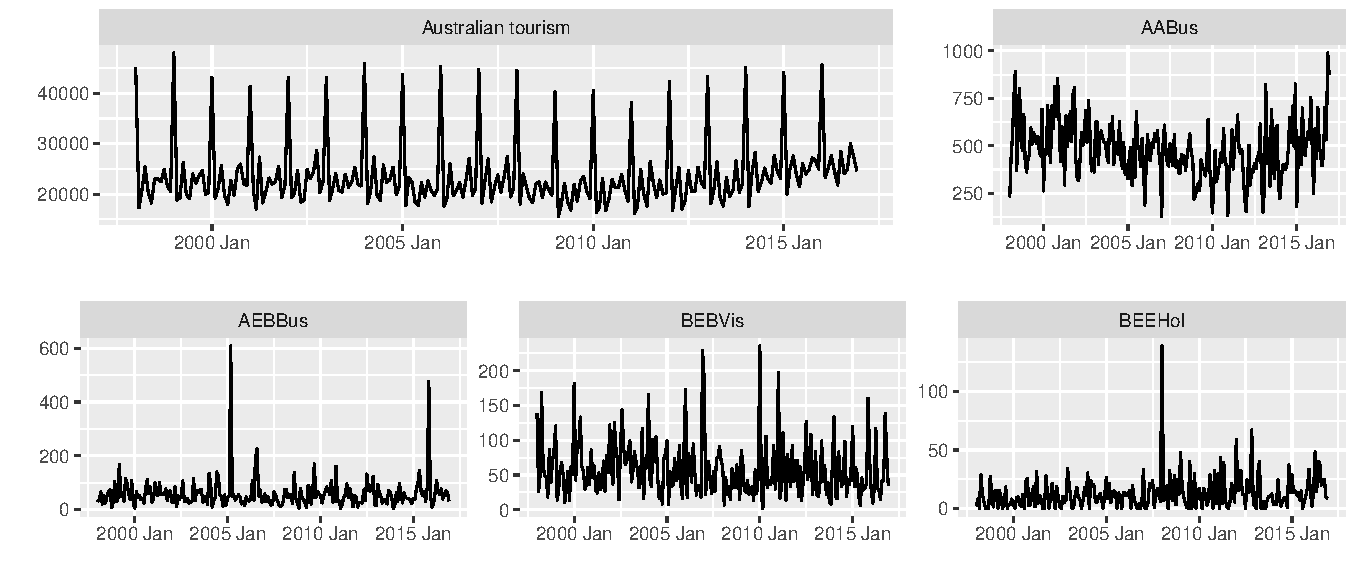
\includegraphics[width=\textwidth]{figures/tourism.pdf}
    \caption{Visualization of selected time series from the tourism dataset. ``AEB'', ``BAB'', ``BEB'', and ``BEE'' represent the regions `New England North West`, `Peninsula', `Western Grampians` and ``Spa Country'', respectively. ``Bus'', ``Oth'', ``Vis'' and ``Hol'' denote travel purposes ``Business'', ``Other'', ``Visit'' and ``Holiday'', respectively.}
    \label{fig:tourism}
\end{figure}

\begin{figure}
    \centering
    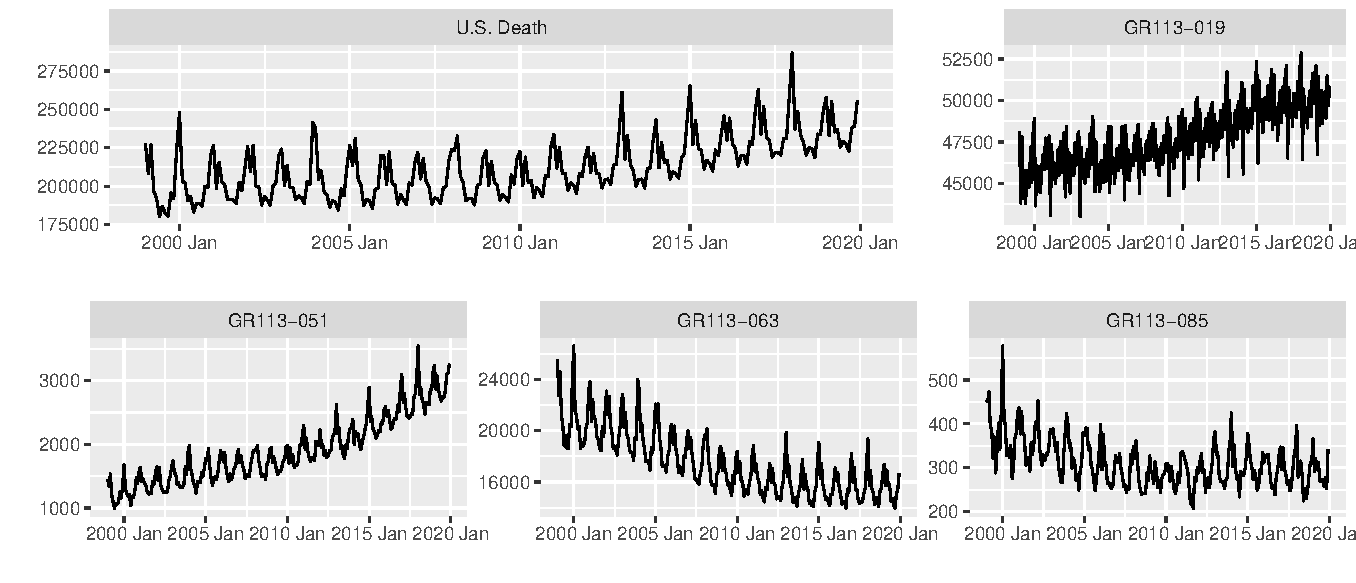
\includegraphics[width=\textwidth]{figures/mortality.pdf}
    \caption{{Visualization of selected time series from the death count dataset.} ``GR113-051'',  ``GR113-063'', ``GR113-085'', and ``GR113-091'' denote ``Parkinson disease'', ``All other forms of chronic ischemic heart disease'', ``Asthma'', and ``Diseases of appendix'', respectively.}
    \label{fig:mortality}
\end{figure}

\subsection{Trace minimization forecast reconciliation approach}


In this subsection, we describe the process of generating coherent forecasts using the trace minimization (MinT) reconciliation approach \citep{wickramasuriyaOptimalForecastReconciliation2019}, which will be employed throughout this paper. Consider a given hierarchy with $n$ time series and $m$ of them being in the bottom level.  Let vectors $\boldsymbol{b}_t$, $\boldsymbol{a}_t$, and $\boldsymbol{y}_t$ represent observations of the bottom level, the aggregated levels (\textit{i.e.} middle and top levels), and the entire hierarchy at time $t$, respectively.
They are linked through an $n\times m$ summing matrix $\boldsymbol{S}$, which can be decomposed into an identity matrix $\boldsymbol{I}_m$ and a constraint matrix $\boldsymbol{A}$ consisting of $0$ and $1$, such that, 
\[
  \boldsymbol{y}_t = \boldsymbol{S}\boldsymbol{b}_t = \begin{bmatrix}
    \boldsymbol{A} \\ \boldsymbol{I}_m 
  \end{bmatrix}  \boldsymbol{b}_t = \begin{bmatrix}
      \boldsymbol{a}_t \\ \boldsymbol{b}_t
  \end{bmatrix},
\]
where $\boldsymbol{A}$ represents the mapping from bottom-level time series to aggregated-level time series. 

Assume our objective is to make $h$-step-ahead forecasts based on $T$ historic observations, we would first produce $h$-step-ahead unreconciled (or ``base'') forecasts $\hat{\boldsymbol{y}}_{T+h}$. Note that there are many different ways to compute such forecasts. In this paper, we adopt the Exponential Smoothing (ETS) method, a well-known univariate forecasting model widely used in both academia and industry \citep{ForecastingExponentialSmoothing}. 
The \code{forecast} (\citealp{forecast}) package in {R} (\citealp{R}) is implemented to produce base forecasts for each time series in the hierarchy.
Subsequently, the MinT reconciliation method is applied to produce coherent forecasts:
\[
    \tilde{\boldsymbol{y}}_{T+h} = (\boldsymbol{S}'\boldsymbol{W}_h^{-1}\boldsymbol{S})^{-1}\boldsymbol{S}'\boldsymbol{W}_h^{-1}\hat{\boldsymbol{y}}_{T+h},
\]
where $\boldsymbol{W}_h$ is the covariance matrix of $h$-step-ahead forecast errors, which is estimated using the MinT shrinkage estimator based on the in-sample one-step-ahead forecast errors (\citealp{wickramasuriyaOptimalForecastReconciliation2019}). 

%\subsection{Grouping-based forecast reconciliation}
\subsection{Augmenting hierarchical time series through clustering}

%DELETE

%Instead of a We use the term ``augmentation'' to denote the process of creating middle-level series by aggregating subsets of bottom-level series. leading to a modified hierarchical time series $\boldsymbol{y}^c_t$, which can be represented as:
%leading to a modified hierarchical time series $\boldsymbol{y}^c_t$, which can be represented as:
%\[
%   \boldsymbol{y}^c_t = \boldsymbol{S}^c\boldsymbol{b}_t = \begin{bmatrix}
%        \boldsymbol{A}' &
%        \boldsymbol{C}_1 &
%        \cdots &
%        \boldsymbol{C}_K &
%        \boldsymbol{I}_m
    %\end{bmatrix}'\boldsymbol{b}_t,
%\] 
%where each $\boldsymbol{C}_k$ represents a newly created middle-level series, formed by aggregating a subset of bottom-level series $\boldsymbol{b}_t$. The vector $\boldsymbol{C}_k$ is of $m$-dimensional and its elements $c_{k, i} \in \{0, 1\}, i=1,\dots m$ indicate whether the $i$-th bottom-level series belongs to the aggregated subset. Notably, different augmentation approaches can result in different hierarchies with varying numbers of new middle-level series $K$. 

%After new hierarchies are constructed, we produce $h$-step-ahead base forecasts based on $T$ observations for each time series in the new hierarchy, and apply forecast reconciliation with MinT shrinkage estimator to obtain reconciled forecasts $\tilde{\boldsymbol{y}}^c_{T+h}$. Given our specific interest in the performance of the two-level hierarchy, we extract reconciled forecasts of the two-level hierarchy from $\tilde{\boldsymbol{y}}_{T+h}^c$, \textit{i.e.},
%\[
%  \tilde{\boldsymbol{y}}_{T+h} = \tilde{\boldsymbol{y}}^c_{T+h, 1:(n-m) \cup (n + K - m + 1): (n+K)}.
%\]

%\subsection{Cluster hierarchy construction approach}

To the best of our knowledge, the following studies are the exclusive examples in the literature that propose to integrate forecast reconciliation with hierarchy construction via time series clustering.
\cite{pangHierarchicalElectricityTime2018} detect consumption patterns of electricity smart meter data based on X-means clustering algorithm, while \cite{pangHierarchicalElectricityTime2022} propose a multiple alternative clustering method to group similar electricity and solar power time series. 
\cite{liForecastReconciliationApproach2019} apply agglomerative clustering to cause-of-death time series, and
\cite{matteraImprovingOutofSampleForecasts2023} utilize Partition Around Medoids algorithms to unveil underlying structures in stock price indexes. 
These studies demonstrate superior forecast performance of the clustering-based hierarchies compared to the natural hierarchy or the two-level hierarchy.
However, these studies are limited in scope as they focus on a small number of  clustering techniques. 
%construct hierarchies through clustering algorithms and 


Inspired by the comprehensive overview of time series clustering by \cite{aghabozorgiTimeseriesClusteringDecade2015a}, we consider various approaches based on three key components, namely time series representations, distance measures, and clustering algorithms. Our framework for creating a clustering approach is as follows: we first choose a time series representation, which can be the raw time series, the in-sample forecast error, features of the time series, or features of the in-sample forecast error. We then select a distance measure, either Euclidean distance or dynamic time warping. Once the representation and the distance measure are determined, we choose a clustering algorithm, either $k$-medoids or agglomerative hierarchical clustering, to form clusters in the dataset. In total, we consider 12 different clustering approaches in our experiments.
%, and evaluation measures. 





% Time series clustering is an essential technique that finds applications across various domains, including finance (\citealp{DIAS2015852}), energy (\citealp{pangHierarchicalElectricityTime2018}), robotics (\citealp{gopalapillaiExperimentationAnalysisTime2014}), and others. It is commonly used to identify similar patterns within time series datasets, aiding in applications such as anomaly detection, pattern discovery, and recommendation.

\subsubsection{Time series representations}


The first step of time series clustering is to find appropriate time series representations. Time series representations transform time series data into another space through techniques like feature extraction or dimension reduction. By utilizing diverse time series representations, we are able to obtain distinct clusters which offer varied perspectives on the same dataset.
Considering the impracticality of exploring every conceivable time series representation, we focus on four key ones: raw time series without any transformation (hereafter referred to as ``time series''), in-sample one-step-ahead forecast error, features of time series, and features of in-sample one-step-ahead forecast error.
The inclusion of raw time series is motivated by its simplicity and broad applicability.
A crucial element contributing to the success of the MinT method lies in estimating the covariance matrix of base forecast errors based on in-sample one-step-ahead forecast error. Hence, we consider in-sample one-step-ahead forecast error as a representation to examine how the structure within the error series influences reconciliation performance. 
Raw time series and in-sample error representations are standardized to eliminate the impact of scale variations. This is done by normalizing each series by subtracting its mean and then dividing by the standard error.

Features, widely employed in capturing time series characteristics across literature, play a pivotal role in various time series applications, including clustering (\citealp{tianoFeatTSFeaturebasedTime2021}) and forecasting (\citealp{wangUncertaintyEstimationFeaturebased2022, liFeaturebasedIntermittentDemand2023}). In our exploration, we incorporate features of both raw time series and in-sample forecast error as representations. The included time series features, calculated by the \code{tsfeatures} (\citealp{tsfeatures}) in R, have been applied in several feature-based forecasting studies, \textit{e.g.}, \cite{montero-mansoFFORMAFeaturebasedForecast2020}.
Notably, to the best of our knowledge, we are the first to utilize in-sample forecast error and time series features as representations in the context of forecast reconciliation literature.
These representations allow us to gain insights into the diverse aspects of hierarchical time series data.




\subsubsection{Distance measures}

Distance measures serve as crucial tools for assessing the similarity/dissimilarity between two series, significantly influencing the clustering results.
We consider two widely applied distance measures: Euclidean distance and dynamic time warping (DTW). Due to the limited number of time series in comparison to the high dimensionality of individual time series (\textit{i.e.}, the length of time series and the number of time series features) in our applications, dimension reduction on the aforementioned representations becomes imperative when employing Euclidean distance. Failure to undertake dimension reduction may result in undesirable clustering outcomes due to the curse of dimensionality. To address this, we perform Principal Component Analysis (PCA), extracting the first few principal components that collectively explain at least 80\% of the variance within the representations.

In contrast, DTW (\citealp{sakoeDynamicProgrammingAlgorithm1978}), exhibits reduced sensitivity to the curse of dimensionality. Unlike Euclidean distance, which performs one-to-one point comparisons, DTW accommodates time series of varying lengths through many-to-one comparisons. This flexible approach allows for the recognition of time series with similar shapes, even in the presence of signal transformations such as shifting and/or scaling.


\subsubsection{Clustering algorithms}
Clustering algorithms, such as partitioning, hierarchical, grid-based, model-based clustering, among others, identify clusters by optimizing specific objective functions (\citealp{aghabozorgiTimeseriesClusteringDecade2015a}). These functions are calculated based on chosen time series representations and distance measures.
In this paper, we focus on two prevalent approaches, $k$-medoids and agglomerative hierarchical clustering. The $k$-medoids algorithm, a classical partitioning clustering method, aims to minimize the total distance between all samples within a cluster and their respective cluster centers. 
Unlike $k$-means which employs the mean vector of samples as the cluster center, $k$-medoids selects one sample within the cluster as the center. 
Specifically, we adopt the $k$-medoids variant, partitioning around medoids (PAM, \citealp{PartitioningMedoidsProgram1990}).
Following the recommendation of \cite{PartitioningMedoidsProgram1990}, we determine the optimal number of cluster using the average silhouette width (ASW), a popular cluster validation index.
ASW assesses the quality of clustering results by measuring the proximity of samples within a cluster compared to neighboring clusters.
Given a clustering result, the silhouette width for the $i$th sample is calculated as 
\[
  SW(i) = \frac{b(i)-a(i)}{\max\{a(i), b(i)\}},  
\]
where $a(i)$ represents the average distance of the $i$th sample to others in the same cluster, and $b(i)$ is the average distance to samples in the nearest cluster it is not assigned to. A higher silhouette width indicates greater proximity to samples within the same cluster than to those in neighboring clusters. The ASW is the average of silhouette widths across all samples. We select the clustering result that maximizes the ASW by iterating over all possible numbers of clusters. However, ASW has the limitation of being undefined when there is only one cluster. 

On the other hand, agglomerative hierarchical clustering begins by considering each sample as a cluster, and then gradually merges clusters until all samples forms a single cluster. Recall that $m$ represents the number of bottom level series. 
This process results in a binary hierarchical tree with ($2m-1$) nodes. We employ Ward's linkage (\citealp{murtaghWardHierarchicalAgglomerative2014a}) to merge clusters, minimizing the increase of within-cluster variances at each step. 

\begin{figure}[h!]
    \centering
    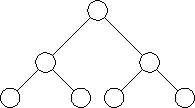
\includegraphics[width=0.45\textwidth]{figures/pamcluster.pdf}
    \hspace{1cm}
    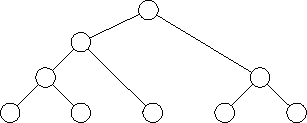
\includegraphics[width=0.45\textwidth]{figures/aggcluster.pdf}
    \caption{\label{fig:cluster_example}Example clustering results of two clustering algorithms. Left panel displays example for $k$-medoids algorithm, and right panel displays example for agglomerative hierarchical clustering algorithm.}
\end{figure}
Illustrated in Figure~\ref{fig:cluster_example} are two example hierarchies generated by $k$-medoids and agglomerative clustering algorithms for an original hierarchy with four bottom-level series and one total series. These examples highlight the distinct behaviors of the two algorithms.
Firstly, $k$-medoids constructs a simple hierarchy with a single middle level, while hierarchical clustering generates multiple nested middle levels. 
Secondly, $k$-medoids produces a hierarchy with the same number of series as the optimal number of clusters, whereas hierarchical clustering yields multiple middle levels with ($m-2$) series.
As the number of bottom-level series increases, the structural differences become increasingly significant, and we aim to investigate how these differences influence the performance of forecast reconciliation.




In summary, we employ 12 time series clustering approaches which are derived from combinations of four time series representations, two distance measures, and two clustering algorithms. The names and details of these approaches are listed in Table~\ref{tab:P3_methods}. The four time series representations need to perform dimension reduction when using Euclidean distance. Combing the four dimension reduced representations with two clustering algorithms results in the first eight clustering approaches. Note that features of raw time series and in-sample forecast error are not temporal data, thus incompatible with DTW. Therefore, the last four approaches are derived from combinations of two temporal representations (\textit{i.e.}, raw time series and in-sample error), DTW, and two clustering algorithms. After filtering out the features that are constant across all series, $56$ features are reserved. The list and descriptions of features are available in the supplementary materials. The $k$-medoids and hierarchical clustering algorithms are implemented using the \texttt{cluster} (\citealp{cluster}) package in R.

\begin{table}[h!]
\caption{\label{tab:P3_methods} Details of the 12 clustering approaches considered.}
\centering
\resizebox{\textwidth}{!}{
\begin{tabular}{lcrrr}
    \toprule
    Approaches & Dimension reduction & Representation & Distance measure & Clustering algorithms  \\ \midrule
    TS-EUC-ME &  Yes & Time series  & Euclidean & $k$-medoids \\
    ER-EUC-ME & Yes& In-sample error  & Euclidean & $k$-medoids \\
    TSF-EUC-ME & Yes& Time series features  & Euclidean & $k$-medoids \\
    ERF-EUC-ME & Yes& In-sample error features  & Euclidean & $k$-medoids \\
    TS-EUC-HC & Yes& Time series  & Euclidean & hierarchical   \\ 
    ER-EUC-HC & Yes& In-sample error  & Euclidean & hierarchical   \\ 
    TSF-EUC-HC & Yes& Time series features  & Euclidean & hierarchical   \\ 
    ERF-EUC-HC & Yes& In-sample error features  & Euclidean & hierarchical  \\
    TS-DTW-ME & No& Time series  & DTW & $k$-medoids \\
    TS-DTW-HC & No& In-sample error  & DTW & hierarchical  \\
    ER-DTW-ME & No& Time series  & DTW & $k$-medoids \\
    ER-DTW-HC & No& In-sample error  & DTW & hierarchical 
     \\\bottomrule
\end{tabular}}
\end{table}



\subsection{Evaluation of forecast accuracy}
\label{subsec:evaluation}

We investigate the impact of clustering on forecast reconciliation via a systematic comparison of the forecast accuracy based on different hierarchies. 
%time series clustering techniques in Table \ref{tab:P3_methods}. %This comparison incorporates a diverse set of time series representations, distance measures, and clustering algorithms to provide a more thorough understanding of their impact on forecast performance.\\
To evaluate the accuracy of reconciled forecasts based on a given hierarchical structure, we first calculate Root Mean Squared Scaled Error (RMSSE, \citealp{makridakisM5AccuracyCompetition2022}) for each series. 
RMSSE is symmetric, independent of the data scale, and thus suitable for evaluating hierarchical forecasts (\citealp{athanasopoulosEvaluationHierarchicalForecasts2023}). 
It is defined as follows:
\[
RMSSE = \sqrt{\frac{\frac{1}{h}\displaystyle\sum_{t=T+1}^{T+h}(y_t-\hat y_{t})^2}{\frac{1}{T-12}\displaystyle\sum_{t=13}^T (y_t - y_{t-12})^2}},
\]
where $\hat y_t$ is the reconciled forecast or base forecast of series $y_t$.
It should be note that the denominator of our RMSSE measure is not exactly same as that in \cite{makridakisM5AccuracyCompetition2022}. We use the in-sample mean squared error of the seasonal naive method because the time series in our applications exhibit monthly seasonality. 
Then, we take average RMSSE of all forecasts in $\tilde{\boldsymbol{y}}_{T+h}$ as measure for the hierarchy.

To rigorously validate our hypothesis, we utilize the rolling window strategy to evaluate the performance of different approaches on both datasets. We begin by producing and evaluating $12$-steps-ahead coherent forecasts using the first $96$ observations. The training set is then increased by one observation and new forecasts are obtained. The procedure is repeated until the last $12$ observations are used for evaluation. Finally, we can obtain $121$ RMSSE (January 2006 - January 2016) for the tourism dataset and $145$ RMSSE (January 2007 - January 2019) for the mortality dataset.  Two approaches are utilized to compare and present the performance of various approaches on two datasets. The first one is to calculate average RMSSE across all evaluation windows, while the second involves Multiple Comparison with the Best (MCB) test (\citealp{koningM3CompetitionStatistical2005}), which computes the average ranks of different approaches across all evaluation windows and assess whether they are statistically different. 


\section{Natural hierarchy}\label{sec:natural}

\subsection{Natural hierarchy vs two-level hierarchy}
\label{subsec:n_vs_twolevel}
In this subsection, we compare the performance of the natural hierarchy against the two-level hierarchy to address the first research question. We expect that natural hierarchy would demonstrate superior performance over the two-level hierarchy, as more time series are included in the reconciliation process.
Following the evaluation procedure introduced in Section~\ref{subsec:evaluation}, Table~\ref{tab:P1} compares forecast accuracy of the natural hierarchy and the two-level hierarchy on tourism and mortality datasets. Average RMSSE is calculated across all evaluation windows. 
%in terms of average RMSSE across all evaluation windows. 
The asterisk in table indicates significant difference according to MCB test.
Table~\ref{tab:P1} shows that natural hierarchy significantly outperforms the two-level hierarchy on both datasets.  It confirms our hypothesis that natural hierarchy improves forecast performance over a two-level hierarchy.

\begin{table}[h!]
    \centering
    \caption{\label{tab:P1} Performance of natural and two-level hierarchies in terms of average RMSSE ($\times 10^{-2}$) across all evaluation windows on both datasets. Column-wise minimum values are displayed in bold. Asterisk (*) indicates significant difference according to MCB test.}
    \begin{tabular}{lll}
    \toprule
        Method & tourism & mortality \\ \midrule
        Natural & $\bold{69.13}^*$ & $\bold{75.01}^*$ \\ 
        Two-level & $69.43$ & $75.28$ \\ \bottomrule
    \end{tabular}
    
\end{table}



\subsection{Permutation of the natural hierarchy}
\label{subsec:permutation}

There are two potential contributors to the improvement in accuracy achieved by the natural hierarchy. First, natural hierarchy could tend to group time series with similar attributes together. 
It is possible that these series share similar trend and seasonality pattern, similar features, strong correlations, or others, resulting in middle-level series with strong signals and easy to forecast.
Thus, total and bottom-level series can borrow strength from these middle-level series during reconciliation. 
We refer to this aspect as ``grouping''.
Second, there are more series and more base forecasts to be combined during reconciliation, which leads to reduced uncertainty (\citealp{petropoulosExploringSourcesUncertainty2018a}) and improved reconciled forecasts. How the series are grouped is however irrelevant. We refer to this aspect as ``structure''. 

To systematically explore these two aspects, we introduce a permutation hierarchy construction method.
Given a hierarchy tree, such as the natural hierarchy, the proposed approach constructs new hierarchies by randomly permuting the leaves. Recall that $\boldsymbol{A}$ is matrix consisting of $0$ and $1$ and represents the mapping from bottom-level time series to aggregated-level time series. In other words, it shuffles the columns of the constraint matrix $\boldsymbol{A}$ of the given hierarchy. This method yields random ``twin'' hierarchies with the same tree structure but different groupings. 
By generating forecasts using the twin hierarchies, we are able to eliminate the influence of grouping and focus specifically on structure. 
If the random twin hierarchies significantly outperform the original counterpart, it suggests that structure holds greater importance than grouping, and vice versa. Figure~\ref{fig:aggcluster_random} shows an example of this approach, where the right hierarchy is a ``twin'' of the left hierarchy.

\begin{figure}
    \centering
    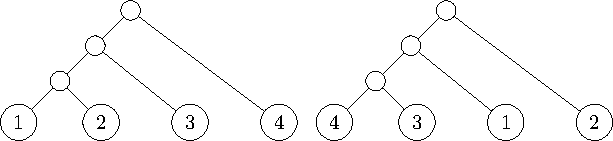
\includegraphics[width=0.8\textwidth]{figures/aggcluster_random.pdf}
    
    \[
    \begin{bmatrix}
    1 & 1 & 1 & 1\\
    1 & 1 & 1 & 0 \\
    1 & 1 & 0 & 0 \\
    & I_4 & & 
    \end{bmatrix}
    \quad
    \rightarrow
    \quad
    \begin{bmatrix}
    1 & 1 & 1 & 1\\
    0 & 1 & 1 & 1 \\
    0 & 1 & 0 & 1 \\
    & I_4 & & 
    \end{bmatrix}
    \]

\caption{\label{fig:aggcluster_random}Examples of permutation of a given hierarchy. Right hierarchy is obtained by shuffling the leaves of left hierarchy. The upper part displays the hierarchy trees, and the lower part displays the corresponding summing matrices.}
\end{figure}


\subsection{Natural hierarchy versus its twins}
\label{subsec:n_vs_pn}

This subsection compares the performance of natural hierarchy and its random twins on mortality and tourism datasets.
For each dataset, we first randomly generate $100$ permutations of the bottom-level series, which are applied to the natural hierarchy, producing $100$ twin hierarchies. Performances of natural hierarchy and its twins are compared using the evaluation process described in Section~\ref{subsec:evaluation}.

Figures~\ref{fig:P2_tourism} and~\ref{fig:P2_mortality} display the MCB test results for the tourism dataset and mortality, respectively. 
In order to save space, we only display the average rank labels for the natural hierarchy and $5$ twins. The grey zone indicates the confidence interval of the average rank of natural hierarchy. Any hierarchy whose confidence interval does not overlap with the grey zone is either significantly better or worse than the natural hierarchy. 

It is immediately clear that across both datasets, the natural hierarchy shows no significant outperformance compared to its random twins. 
On the tourism dataset, it ranks the $5$th, performing indistinguishably from $32$ twins but significantly better than the remaining $68$.
On the other hand, the performance difference is much smaller for the mortality dataset, where most twins perform insignificantly from the natural hierarchy. There are even three twin hierarchies significantly better than natural hierarchy.
These results suggest that the natural hierarchy of tourism dataset may be ``smarter'' compared to that of mortality dataset.


\begin{figure}[!ht]
    \centering
    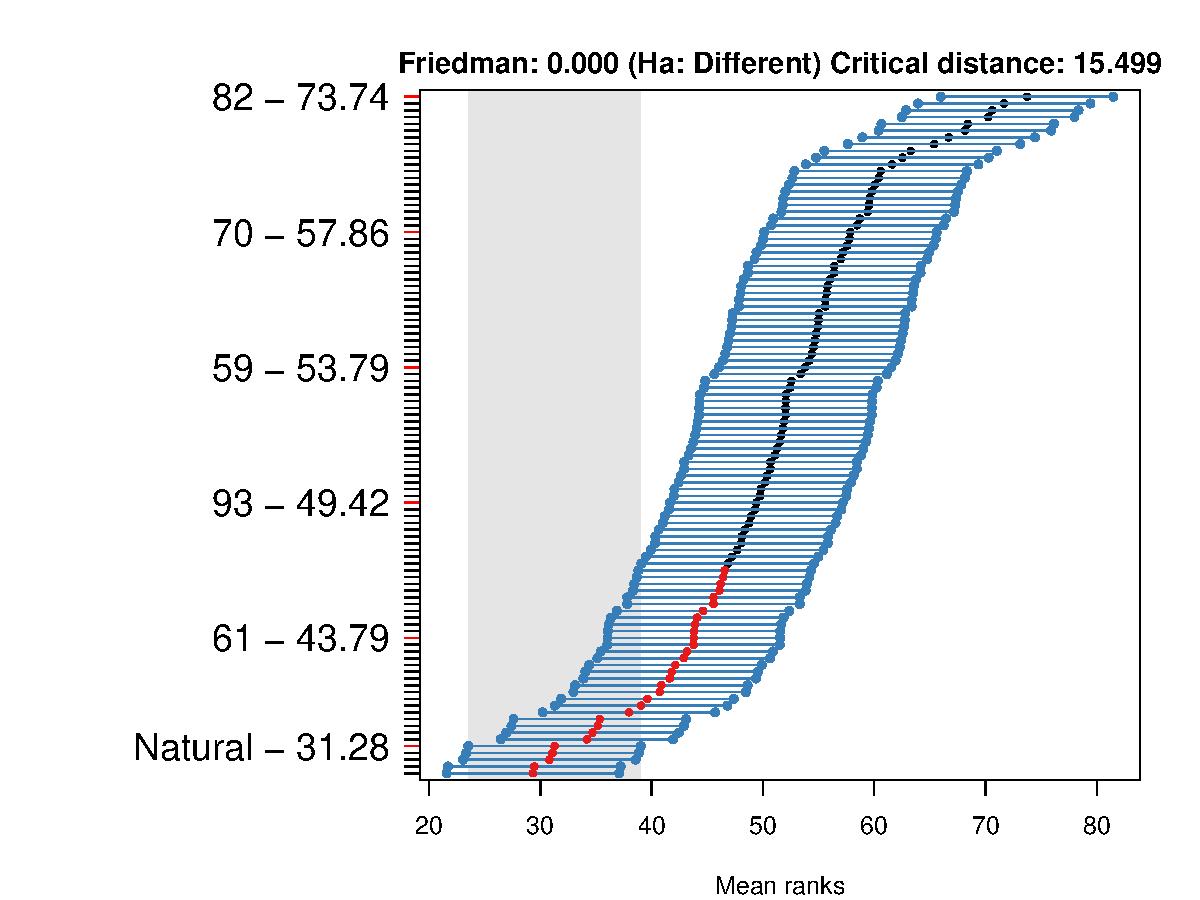
\includegraphics[width=0.8\textwidth]{figures/hierarchy_rmsse/tourism/P2_natural_vs_pn_h12.pdf}
    \caption{\label{fig:P2_tourism}Average ranks and 95\% confidence intervals for natural hierarchy and its $100$ twins on the tourism dataset.}
\end{figure}

\begin{figure}[!ht]
    \centering    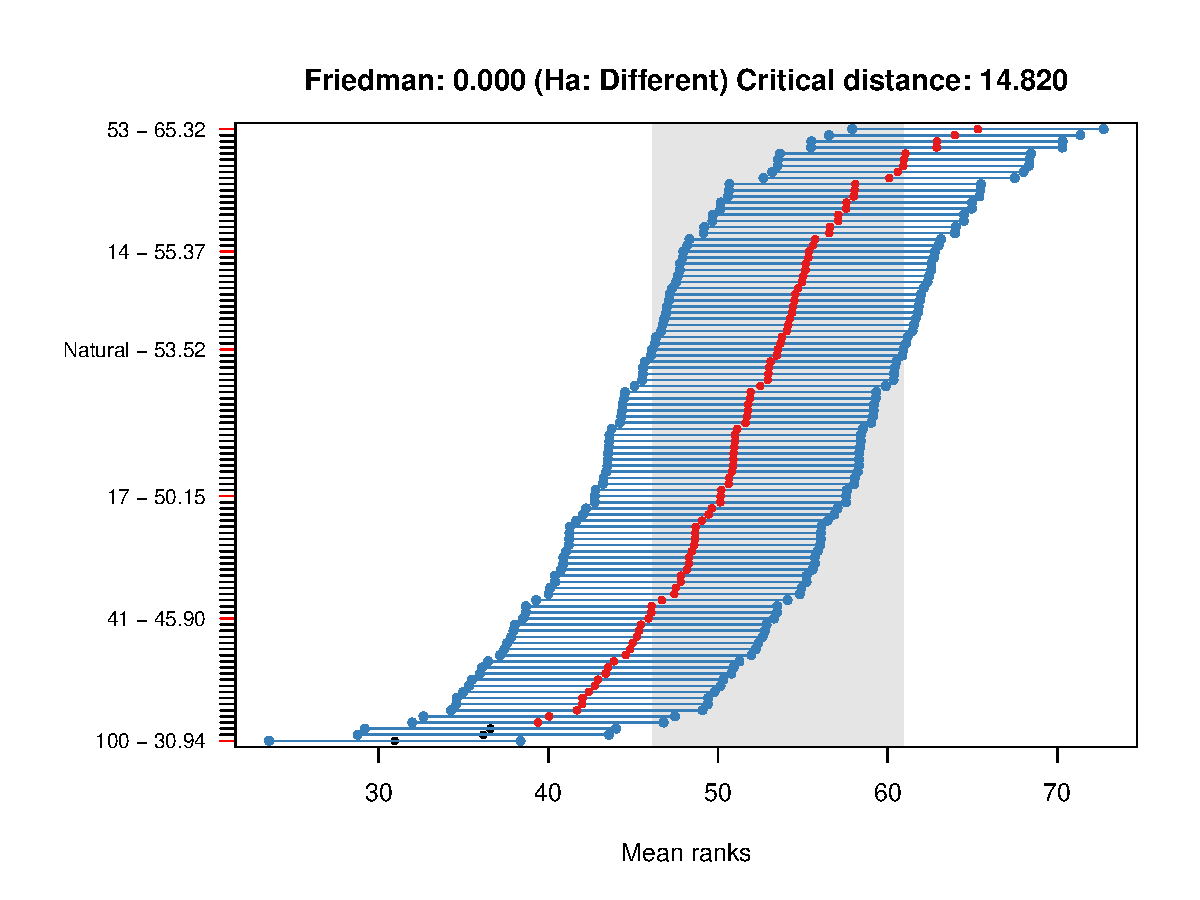
\includegraphics[width=0.8\textwidth]{figures/hierarchy_rmsse/mortality/P2_natural_vs_pn_h12.pdf}
    \caption{\label{fig:P2_mortality}Average ranks and 95\% confidence intervals for natural hierarchy and its $100$ twins on the mortality dataset.}
\end{figure}

\section{Clustering-based hierarchy}
\label{sec:clustering}

Given that ``structure'' of natural hierarchy is the primary contributor to the performance improvement, we are interested in if better groupings can be constructed via clustering and become more critical than structure. 
We first review existing literature on clustering-based forecast reconciliation, and then describe the clustering techniques involved in our paper, followed by empirical results on mortality and tourism dataset.

\subsection{Cluster hierarchies vs benchmarks}
\label{subsec:P3_benchmark}
Table~\ref{tab:P3_rmsse} shows the accuracy of benchmarks and $12$ cluster hierarchies in terms of average RMSSE across all evaluation windows using the evaluation process described in Section~\ref{subsec:evaluation}.  
The MCB test results are presented in Figure~\ref{fig:P3_mcb_benchmark}.
On the tourism dataset, all cluster hierarchies outperform the two-level hierarchy, with ten showing significant improvement.
While on the mortality dataset, only five cluster hierarchies surpass the two-level hierarchy in average RMSSE and eight do so in terms of average ranks. 
However, none of these differences are statistically significant. 
The inferiority of three $k$-medoids based cluster hierarchies highlights the importance of choosing an appropriate clustering technique.
\begin{table}[h!]
    \centering
    \caption{\label{tab:P3_rmsse}Performance of cluster hierarchies and benchmark hierarchies in terms of average RMåSSE($\times 10^{-2}$) across all evaluation windows on both datasets. Column-wise minimum values are displayed in bold.}
    \begin{tabular}{lll}
    \toprule
        Method & tourism & mortality \\ \midrule
        Base & 69.452 & 75.295 \\ 
        Two-level & 69.437 & 75.281 \\ 
        Natural & 69.132 & 75.008 \\ 
        TS-HC-EUC & 69.224 & 75.396 \\ 
        TS-HC-DTW & 69.108 & \textbf{74.959} \\ 
        TS-ME-EUC & 69.392 & 75.279 \\ 
        TS-ME-DTW & 69.404 & 75.278 \\ 
        TSF-HC-EUC & \textbf{69.086} & 75.091 \\ 
        TSF-ME-EUC & 69.385 & 75.488 \\ 
        ER-HC-EUC & 69.196 & 75.068 \\ 
        ER-HC-DTW & 69.121 & 75.324 \\ 
        ER-ME-EUC & 69.380 & 75.303 \\ 
        ER-ME-DTW & 69.420 & 75.308 \\ 
        ERF-HC-EUC & 69.099 & 75.010 \\ 
        ERF-ME-EUC & 69.417 & 75.325 \\ \bottomrule
    \end{tabular}
\end{table}


\begin{table}[!ht]
    \centering
    \caption{\label{tab:P3_features}Four trend and seasonality features for the tourism dataset and mortality dataset.}
    \begin{tabular}{lll}\toprule
        Features & mortality & tourism \\ \midrule
        $\gamma$ parameter of Holt-Winters model & 0.0202 & 0.000165 \\ 
        The first order seasonal ACF & 0.652 & 0.181 \\ 
        Strength of trend & 0.757 & 0.156 \\ \bottomrule
    \end{tabular}
\end{table}

The varying performance of cluster hierarchies across two datasets can be attributed to the unique characteristics of their bottom-level series.
The tourism dataset, as shown in Figure~\ref{fig:tourism}, predominately contains volatile and noisy bottom-level time series with weak trend and seasonality. Creating new middle-level time series in this context helps elucidate the underlying pattern which can not be easily captured by bottom-level base forecasting models. 
On the other hand, bottom-level series in mortality dataset exhibit stronger trend and seasonality patterns, making creating middle-level series less beneficial. Table~\ref{tab:P3_features} summarises several features computed using available data in the last evaluation window, confirming the stronger seasonality and trend presence in the bottom level of mortality dataset. Note that the values are computed by averaging features for all bottom-level time series. The strength of trend is defined as 
\[
\text{Strength of trend} = 1-\frac{\text{Var}(e_t)}{\text{Var}(f_t+e_t)},
\]
where $e_t$ and $f_t$ are residuals component and smoothed trend component obtained by STL decomposition of the time series (\citealp{tsfeatures}).

\begin{table}[h!]
    \centering
    \caption{\label{tab:P3_number_series}Average number of middle-level time series for $k$-medoids-based, hierarchical-clustering-based and natural hierarchy in both datasets.}
    \begin{tabular}{lll}
    \toprule
        Approach & mortality & tourism \\ \midrule
     Natural & 21 & 250 \\ 
        $k$-medoids clustering & 6.78 & 20.99 \\ 
        Hierarchical clustering & 96 & 302 \\ \bottomrule
    \end{tabular}
\end{table}

The hierarchies based on hierarchical clustering outperforms the hierarchies based on $k$-medoids when using the same representation and distance metric, e.g., ``TSF-HC-EUC'' outperforms ``TSF-ME-EUC''.
This superiority is attributed to hierarchical clustering generating a greater number of middle-level time series than $k$-medoids, significantly enhancing the benefits of enriched structure.
Table~\ref{tab:P3_number_series} summarises average number of middle-level series across all evaluation windows for natural, $k$-medoids-based and hierarchical clustering-based hierarchy. 
Interestingly, the natural hierarchy shows competitive accuracy compared to hierarchical clustering-based hierarchies on both datasets, despite having fewer middle-level series.
Regarding the superiority of any specific representation or distance metric, no consistent findings emerge. 
   


\begin{figure}
    \centering
    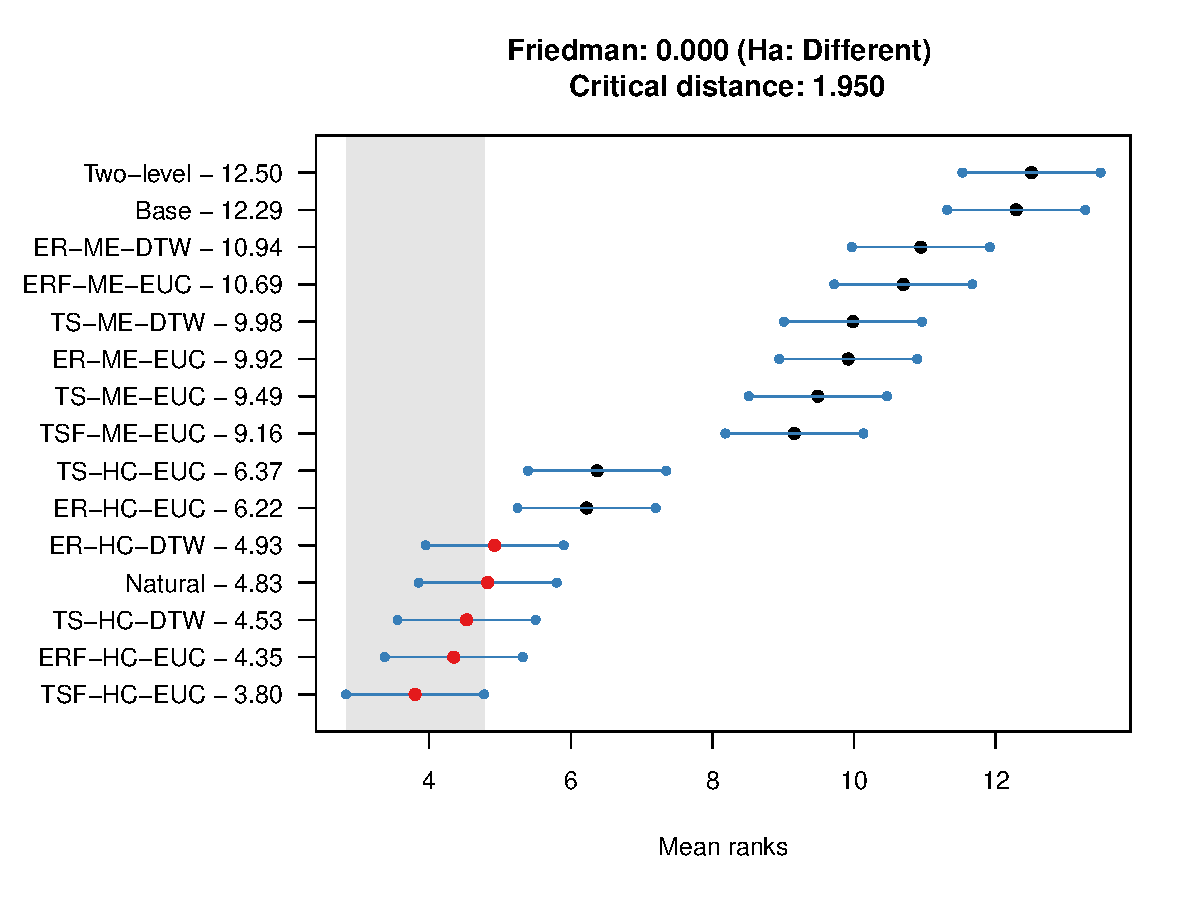
\includegraphics[width=0.45\textwidth]{figures/hierarchy_rmsse/tourism/P3_mcb_benchmarks_h12.pdf}
    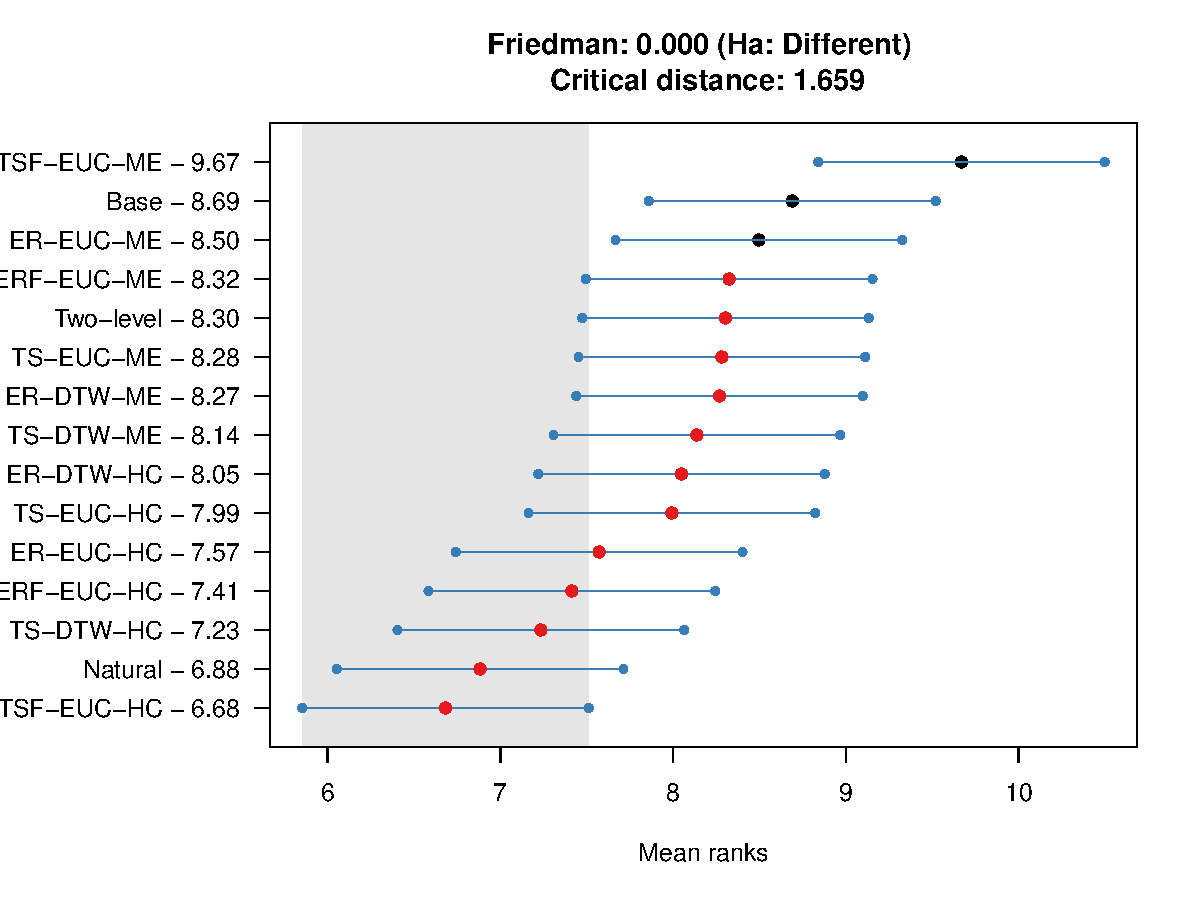
\includegraphics[width=0.45\textwidth]{figures/hierarchy_rmsse/mortality/P3_mcb_benchmarks_h12.pdf}
    \caption{\label{fig:P3_mcb_benchmark}Average ranks and 95\% confidence intervals for twelve cluster hierarchies and three benchmarks on tourism dataset (left) and mortality dataset (right) based on MCB test.}
\end{figure}


\subsection{Cluster hierarchy vs its twins}
\label{subsec:P3_c_vs_pc}

Results in Section~\ref{subsec:P3_benchmark} demonstrate that cluster hierarchy is able to improve forecast performance compared to natural hierarchy and two-level hierarchy. 
We are also interested in how ``structure'' and ``grouping'' contribute to these improvements. Following the comparison in Section~\ref{subsec:n_vs_pn}, we compare the best performing cluster hierarchy with its $100$ random twins. 
Note that we choose the best performing approach according to average RMSSE shown in Table~\ref{tab:P3_rmsse}.

The MCB test results for the tourism dataset and mortality dataset are shown in Figure~\ref{fig:P3_tourism_c_vs_pc} and Figure~\ref{fig:P3_mortality_c_vs_pc}, respectively.
We observe that in both datasets, the best performing clustering approach does not yield significantly better results than its random twins. 
Indicatively, the best cluster approach of mortality dataset ranks nearly in the middle of its random twins, indicating that structure instead of grouping dominates the performance. 
However, the best cluster approach of tourism dataset ranks first and significantly outperforms $70$ of its random twins. This suggests a combination effect of grouping and structure.

Overall, Table~\ref{tab:P3_rmsse}, Figures~\ref{fig:P3_tourism_c_vs_pc} and \ref{fig:P3_mortality_c_vs_pc} suggest that while it is possible to construct a ``smart'' hierarchical structure that improves forecast reconciliation performance, this possibility highly depends on the dataset characteristic and the time series cluster methods employed, making it a challenging objective to achieve. On the other hand, no matter the ``smarter'' hierarchy is construed or not, enriched structure contributes to the performance improvement.


\begin{figure}[!h]
    \centering
    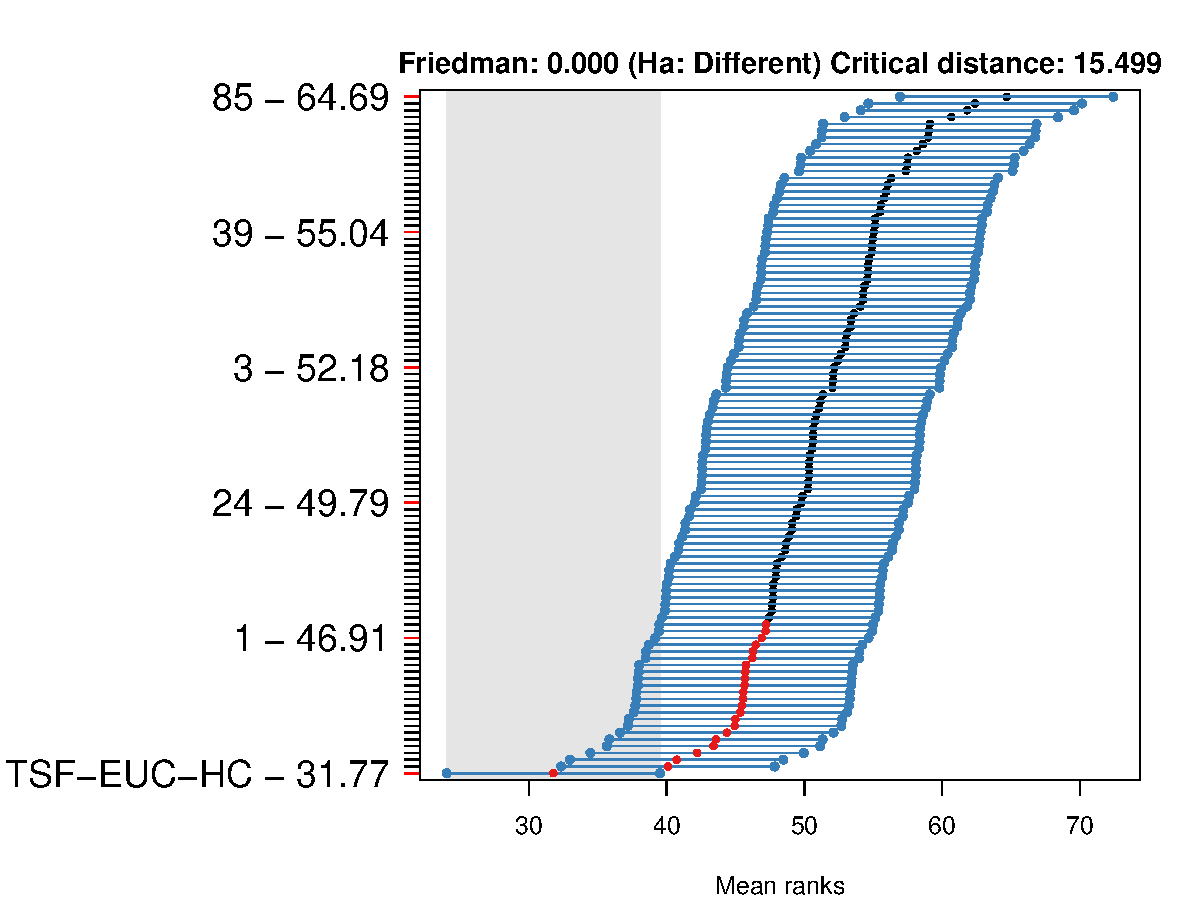
\includegraphics[width=0.7\textwidth]{figures/hierarchy_rmsse/tourism/P3_cluster_vs_pc_h12.pdf}
    \caption{\label{fig:P3_tourism_c_vs_pc}Average ranks and 95\% confidence intervals for best performing cluster hierarchy TSF-HC-EUC and its $100$ twins on the tourism dataset.}
\end{figure}

\begin{figure}[!h]
    \centering
    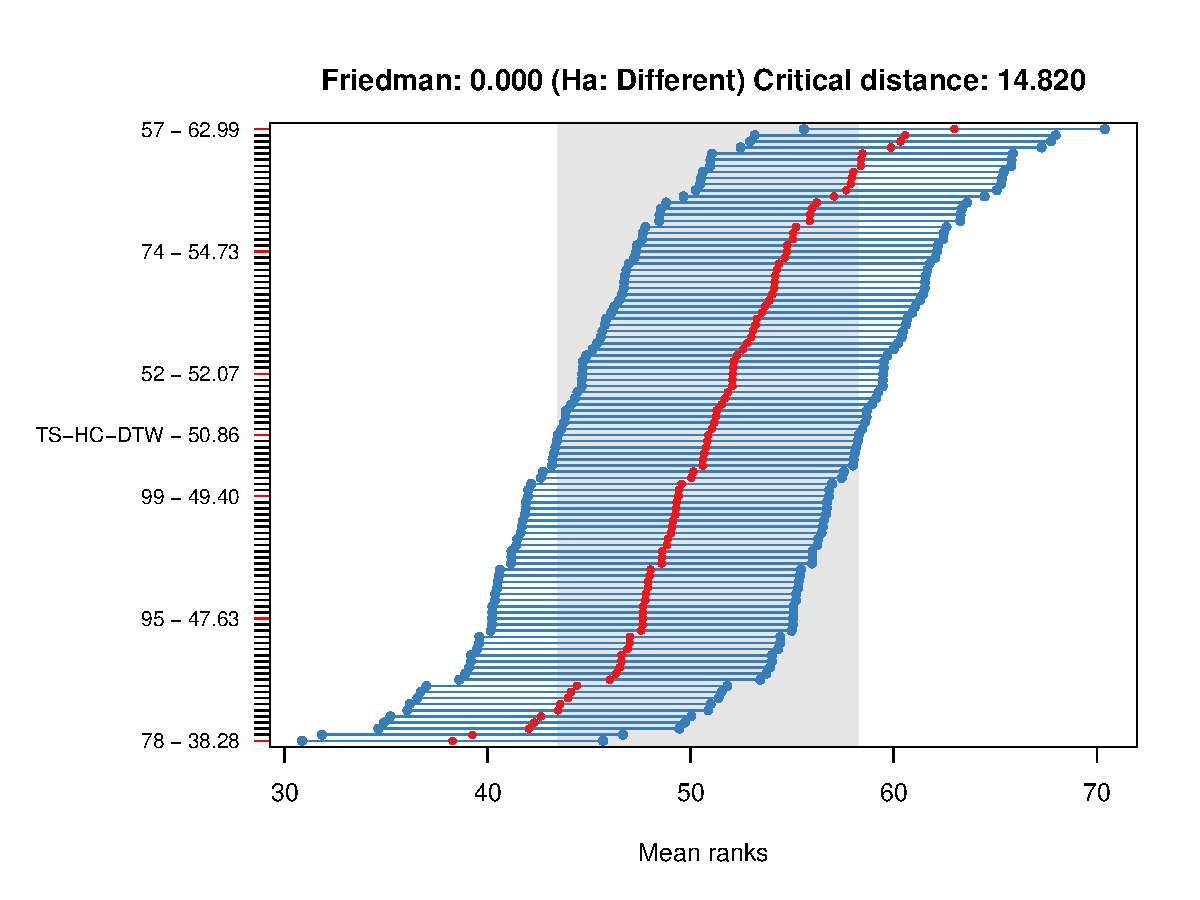
\includegraphics[width=0.7\textwidth]{figures/hierarchy_rmsse/mortality/P3_cluster_vs_pc_h12.pdf}
    \caption{\label{fig:P3_mortality_c_vs_pc}Average ranks and 95\% confidence intervals for best performing cluster hierarchy TS-HC-DTW and its $100$ twins on the mortality dataset.}
\end{figure}



\section{Simulation study}
\label{sec:simulation}

The experiments in Section~\ref{sec:clustering} show the difficulty of constructing a smart hierarchy through clustering. However, it is possible that the clustering approaches we used are unable to detect clusters underlying the dataset. 
In this section, we simulate a scenario where ideal clusters can be detected and investigate how the two factors affect performance in this secenario.


\subsection{Simulation design}

%\subsubsection{Time series generation}

We assume the bottom-level time series follow an additive time series pattern with a data generating process described as follows:
\begin{equation}
    \label{simu:DGP}
    \begin{aligned}
    Y_t &= L_t + S_t + \xi_t \\
    S_t &= S_{t~\text{mod}~s} \\
    L_t &= \alpha t + \varepsilon_t,
    \end{aligned}
\end{equation}
where $L_t$ represents the trend term which increases or decreases over time at a slope of $\alpha$. The seasonal component, denoted by $S_t$, is repeating and deterministic with a cycle of length $s$. Both $\xi_t$ and $\varepsilon_t$ are white noises.


Instead of employing cluster algorithms, we artificially craft $6$ ideal clusters by manipulating the directions of the trend components and patterns of the seasonal components.
The configurations for each cluster can be found in Table~\ref{table:simu_params}. To simulate an increasing trend, we set the slope $\alpha$ to $0.001$, and for a decreasing trend, we set $\alpha$ to $-0.002$. The variances of the associate white noise $\varepsilon_t$ are set to $2.5\times 10^{-5}$ and $4.9\times 10^{-5}$ for increasing trend and decreasing trend, respectively. For series without trend (``None''), the trend component $L_t$ is set to zero. The terms ``Even'' and ``Odd'' in our setup refer to the positioning of seasonal peak. Specifically, ``Even'' seasonality means that peaks occur at even-numbered positions (e.g., $2, 4, \dots$) of seasonal cycle, with the reverse being true for ``Odd'' seasonality. The values of these seasonal peaks and troughs are randomly drawn from uniform distributions within the ranges of $[2, 3]$ and $[0,1]$, respectively. The variance of $\xi_t$ is set to $0.25$. We generate monthly time series data, ensuring that each cluster contains $20$ distinct time series. For each series, we generate $144$ observations, and the last $12$ observations are reserved for evaluation purpose. Figure~\ref{fig:simu_emps} displays example time series from each cluster, while Figure~\ref{fig:simu_pca} visualizes these generated time series based on the first two principal components extracted from principal component analysis of the series.

\begin{table}
\caption{\label{table:simu_params}Parameter setting for all clusters in the simulation experiments.}
\centering
\begin{tabular}{lcccccc}\toprule
& Cluster 1 & Cluster 2 & Cluster 3 & Cluster 4 & Cluster 5 & Cluster 6 \\
Trend & Increase & Increase & None & None & Decrease & Decrease \\
Seasonality & Odd & Even & Odd & Even & Odd & Even  \\
    \bottomrule
\end{tabular}
\end{table}

\begin{figure}
\centering
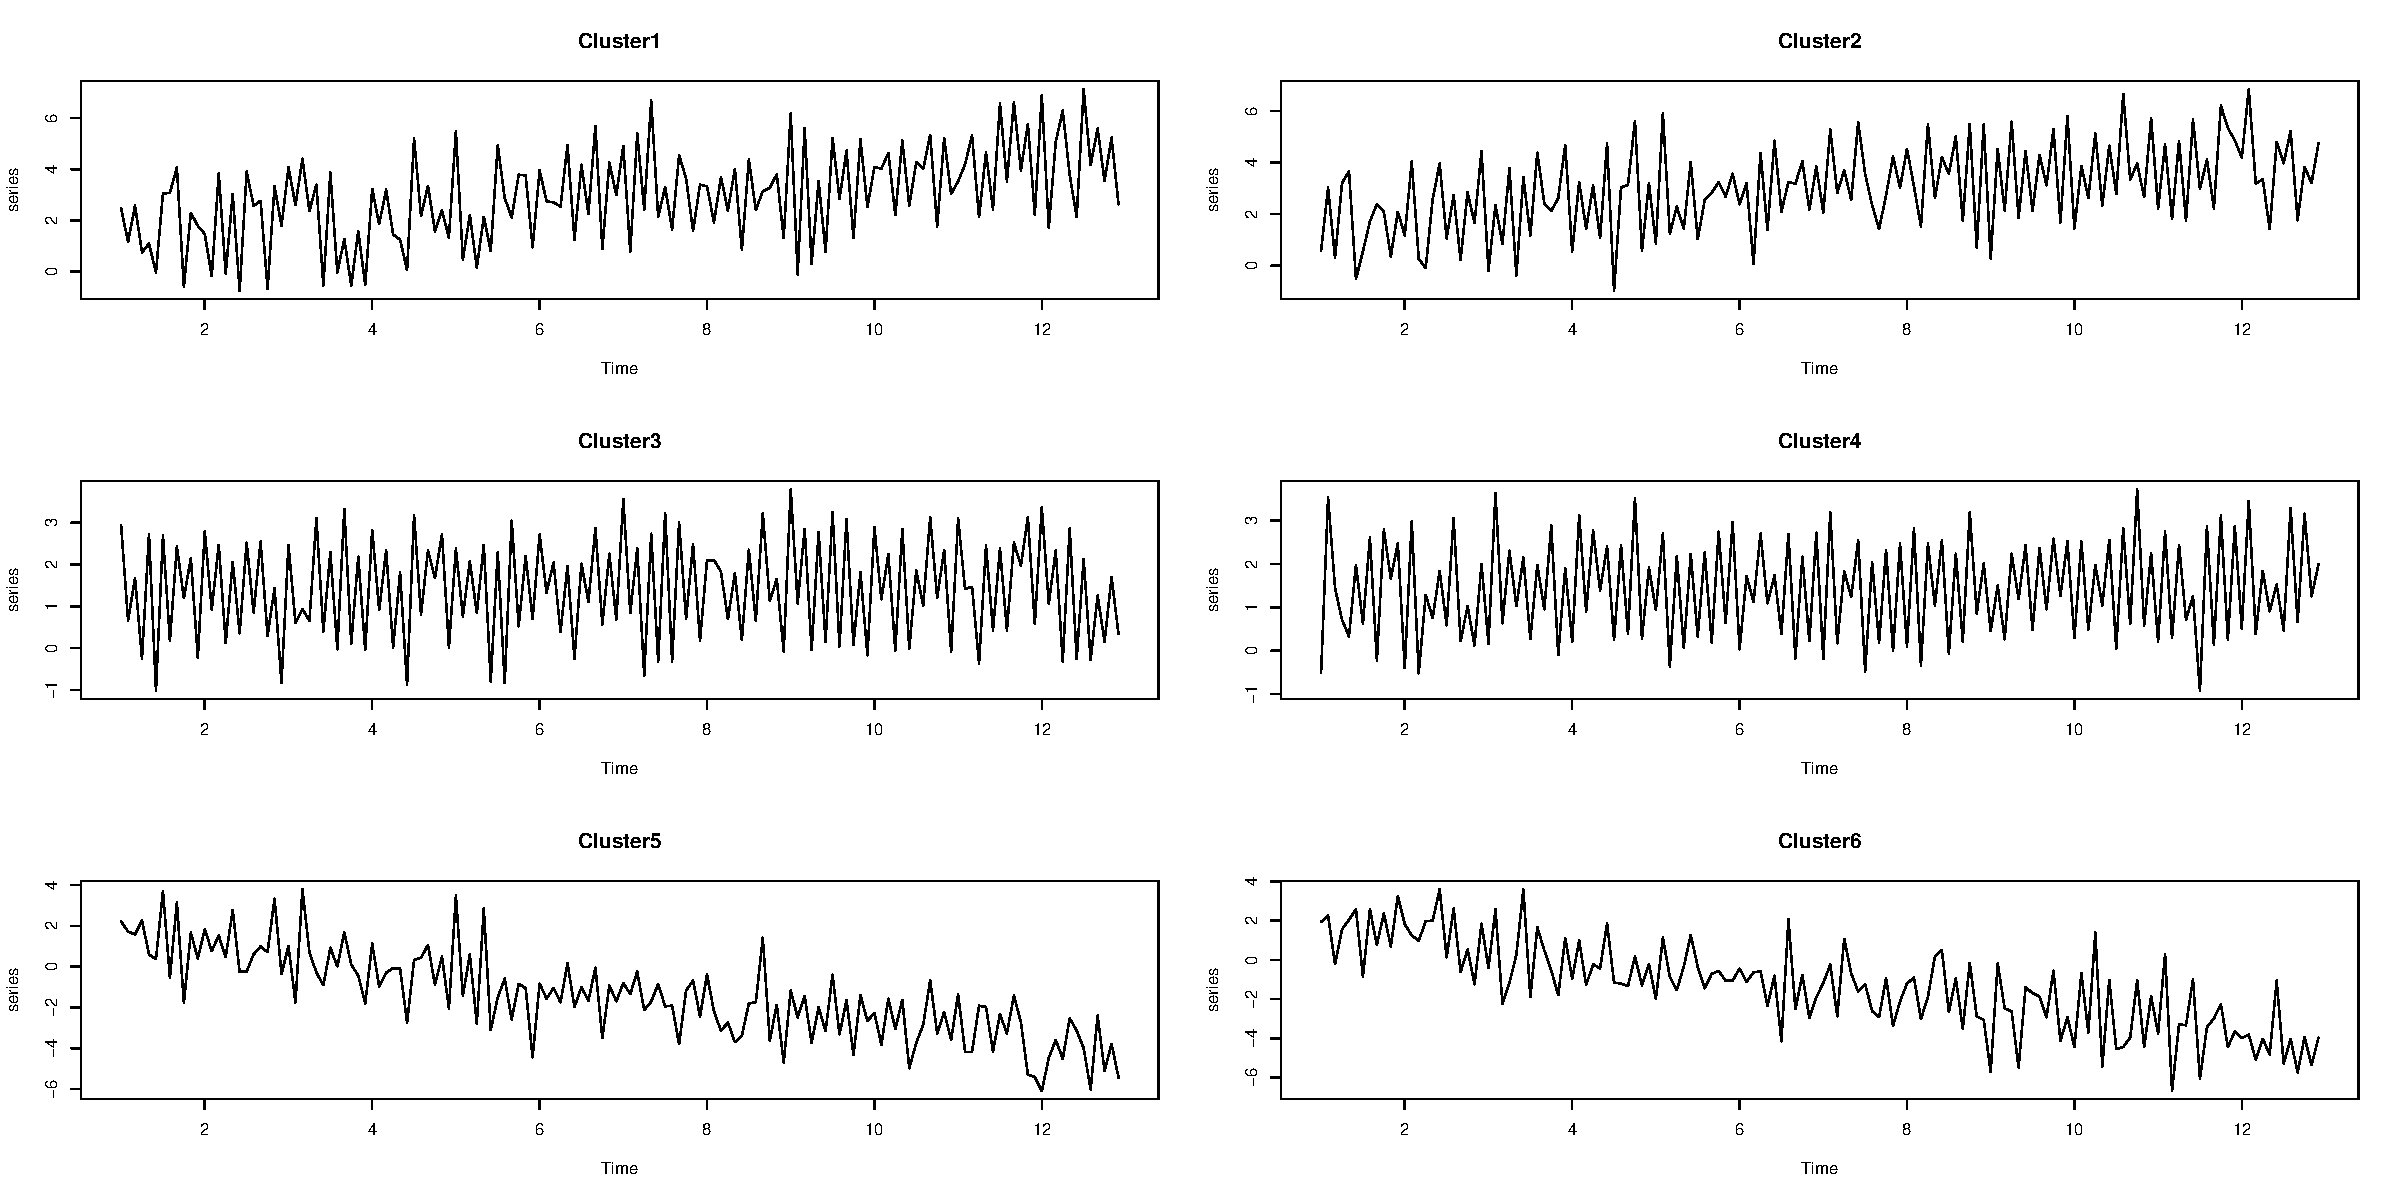
\includegraphics[width=\textwidth]{figures/simu_example.pdf}
\caption{\label{fig:simu_emps}Example time series for each cluster in the simulation experiments.}
\end{figure}

\begin{figure}
    \centering
    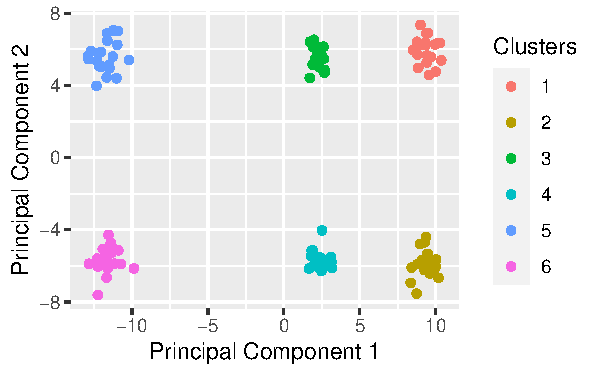
\includegraphics[width=0.6\textwidth]{figures/simu_pca.pdf}
    \caption{\label{fig:simu_pca}Visualization of the generated time series in the simulation experiments.}
\end{figure}

\subsection{Hierarchies construction}

We consider a two-level hierarchy with a total of $120$ bottom-level series and a single aggregated series, labelled as ``Two-level''. In addition, we examine four cluster hierarchies. Note that we consider multiple cluster hierarchies in order to reflect the real-world scenario where a variety of clustering techniques may be employed. The first cluster hierarchy, ``Cluster'', forms six middle-level series according to the predefined ideal clusters. We then merge clusters with the same trend pattern, resulting in the cluster hierarchy with three clusters, denoted by ``Cluster-trend1''. Similarly, we construct cluster hierarchies ``Cluster-trend2'' and ``Cluster-season'' based on the presence of the trend term and seasonal peak positioning, resulting in $2$ and $3$ middle-level series, respectively.
Table~\ref{table:simu_params} summarizes the five approaches.

\begin{table}[]
    \centering
    \begin{tabular}{ll}\toprule
        Approaches & Description \\ \midrule
        Two-level &  The original two-level hierarchy. \\ 
        Cluster & Cluster hierarchy based on ideal clustering. \\
        Cluster-trend1 & Cluster hierarchy based on trend patterns. \\
        Cluster-trend2 & Cluster hierarchy based on existence of trend component. \\
        Cluster-season & Cluster hierarchy based on seasonality patterns. \\\bottomrule
    \end{tabular}
    \caption{\label{tab:simu_methods}Five approaches used in the simulation experiments.}
\end{table}



\subsection{Results}
\label{sec:simu_res}

We repeat the simulation $500$ times and evaluate the results on these $500$ hierarchies following the evaluation procedure introduced in Section~\ref{subsec:evaluation}.
Table~\ref{tab:simu_P3} reports the average RMSSE across all hierarchies, and
Figure~\ref{fig:simu_P3_benchmarks} presents the MCB test results. The results reveal that most approaches perform better than the base forecasts and the original two-level hierarchy. This outcome indicates that hierarchy construction generally improves forecast reconciliation performance, corroborating our findings reported in Section~\ref{sec:clustering}. 
Interestingly, the ideal cluster ``Cluter'' achieves second rank, indicating that optimal clustering does not necessarily translate into the best forecast reconciliation performance. 

Furthermore, we are interested in structure or grouping contributes more to the performance improvements. Again, following the random hierarchy construction procedure described in Section~\ref{subsec:permutation}, we compare the ideal cluster with its $100$ random twins. The MCB test result is shown in Figure~\ref{fig:simu_P3_c_vs_pc}. Even if the optimal cluster can be obtained in this simulation, the results are similar to what we found on the mortality dataset, showing that  structure plays a greater role in improving the forecast reconciliation performance. It enforces our belief that the reason of clustering improving performance depends on the dataset characteristics.


\begin{table}[!ht]
    \centering
    \caption{\label{tab:simu_P3}Performance of cluster hierarchies and benchmark hierarchies in terms of average RMSSE($\times 10^{-2}$) in simulation. Column-wise minimum values are displayed in bold.}
    \begin{tabular}{ll}\toprule
        Method & RMSSE \\ \midrule
        Base & 77.64 \\ 
        Two-level & 59.71 \\ 
        Cluster & 59.63 \\ 
        Cluster-trend1 & \textbf{59.62} \\ 
        Cluster-trend2 & 59.65 \\ 
        Cluster-season & 59.65 \\ \bottomrule
    \end{tabular}
\end{table}

\begin{figure}
    \centering
    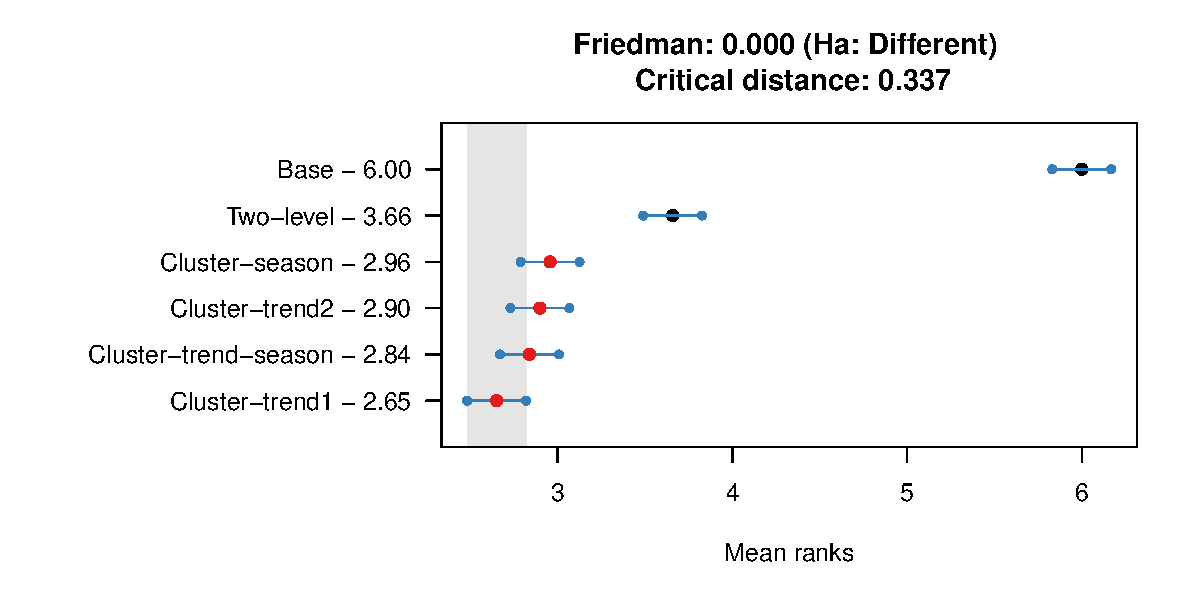
\includegraphics[width=0.6\textwidth]{figures/hierarchy_rmsse/simulation/P3_mcb.pdf}
    \caption{\label{fig:simu_P3_benchmarks}Average ranks and 95\% confidence intervals for four cluster hierarchies and two benchmarks in simulation based on MCB test.}
\end{figure}

\begin{figure}
    \centering
    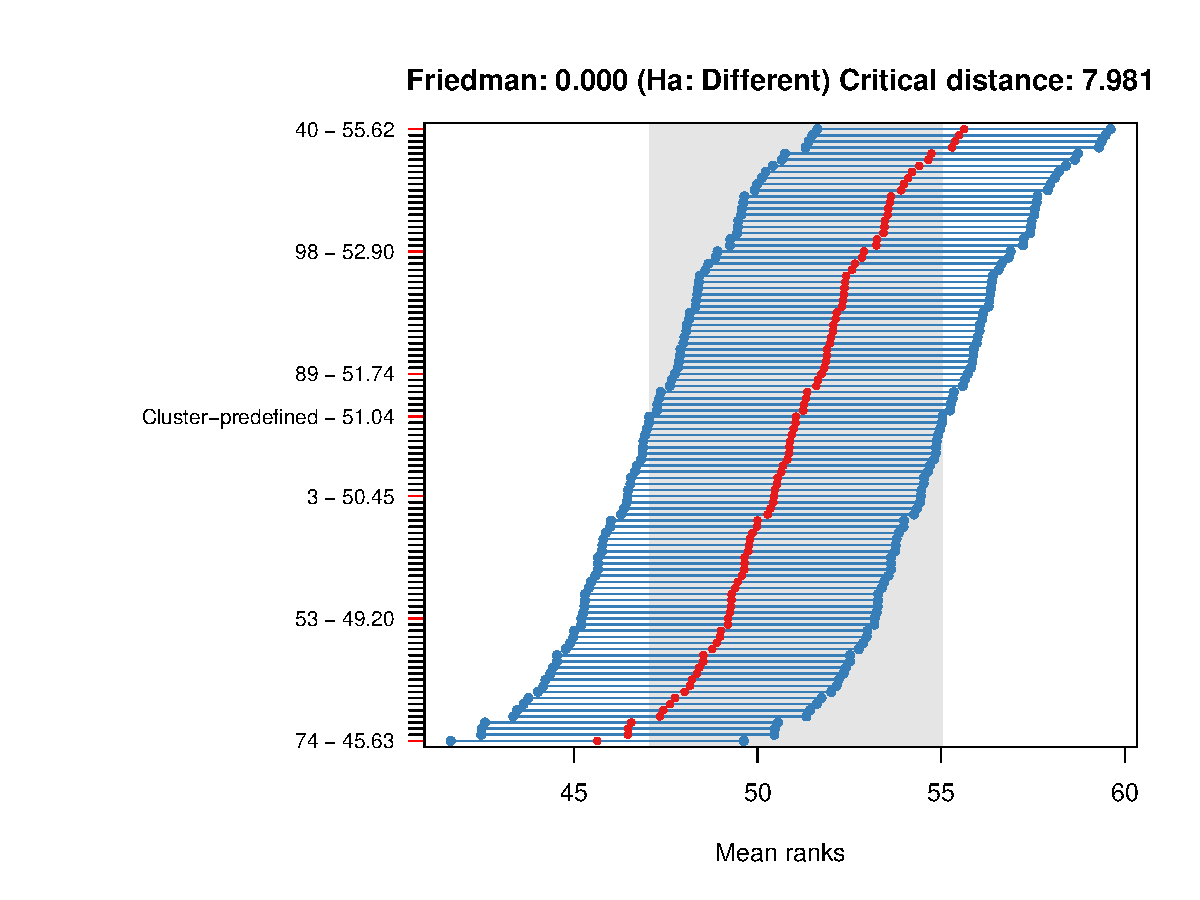
\includegraphics[width=0.8\textwidth]{figures/hierarchy_rmsse/simulation/P3_c_vs_pc.pdf}
    \caption{Average ranks and 95\% confidence intervals for four the ideal hierarchy and its 100 random twins in simulation based on MCB test.}
    \label{fig:simu_P3_c_vs_pc}
\end{figure}



\section{Combination hierarchies}
\label{sec:combination}

The results in Section~\ref{sec:clustering} and Section~\ref{sec:simulation} highlights the possibility of improving forecast reconciliation performance by constructing new middle levels through time series clustering. 
However, this possibility highly depends on the dataset characteristics and time series approaches used.
Therefore, the classical problem of selecting the optimal clustering approaches arises.
Considering the substantial research and empirical evidences in favor of forecast combination over selection (see e.g., \citealp{elliottForecastingEconomicsFinance2016}), we suggest employing combination of forecasts from multiple cluster hierarchies to avoid the uncertainty associated with identifying a best cluster approach.
Specifically, the reconciled forecasts from multiple hierarchies are combined using equal weights, i.e.,
\[
  \tilde{\boldsymbol{y}}_{T+h}^{\text{comb}} = \frac{1}{l} \sum_{j=1}^l \tilde{\boldsymbol{y}}_{T+h}^j.
\] Note that the resulted forecasts are still coherent. 
While it is possible to employ more complex methods to determine ``optimal'' weights, we adhere to equally-weighted combination due to its simplicity and well-known efficacy (\citealp{wangForecastCombinations50year2022}).

Following the evaluation procedure introduced in Section~\ref{subsec:evaluation},
Table~\ref{tab:P4_RMSSE} presents the accuracy in terms of average RMSSE across all evaluation windows for both datasets. Note that we only present accuracies of three benchmarks, the best cluster hierarchies and the combination hierarchy to save space. The MCB test results are shown in Figure~\ref{fig:P4_bench_mcb}. 
As expected, we observe that on both datasets, forecast combination future improves forecast performance compared to the best performing cluster hierarchy. 
The improvement on the mortality dataset is more pronounced, with forecast combination significantly outperforms all other approaches.
\begin{table}[!ht]
    \centering
    \caption{\label{tab:P4_RMSSE}Performance in terms of average RMSSE($\times 10^{-2}$) on both datasets. Column-wise minimum values are displayed in bold.}
    \begin{tabular}{lcc}\toprule
        Method & tourism & mortality \\ \midrule
        Base & 69.452 & 75.295 \\ 
        Two-level & 69.437 & 75.281 \\ 
        Natural & 69.132 & 75.008 \\ 
        TS-HC-DTW & 69.108 & 74.959 \\ 
        TSF-HC-EUC & 69.086 & 75.091 \\ 
        Combination & \textbf{69.019} & \textbf{74.234} \\ \bottomrule
    \end{tabular}
\end{table}

\begin{figure}[!h]
    \centering
    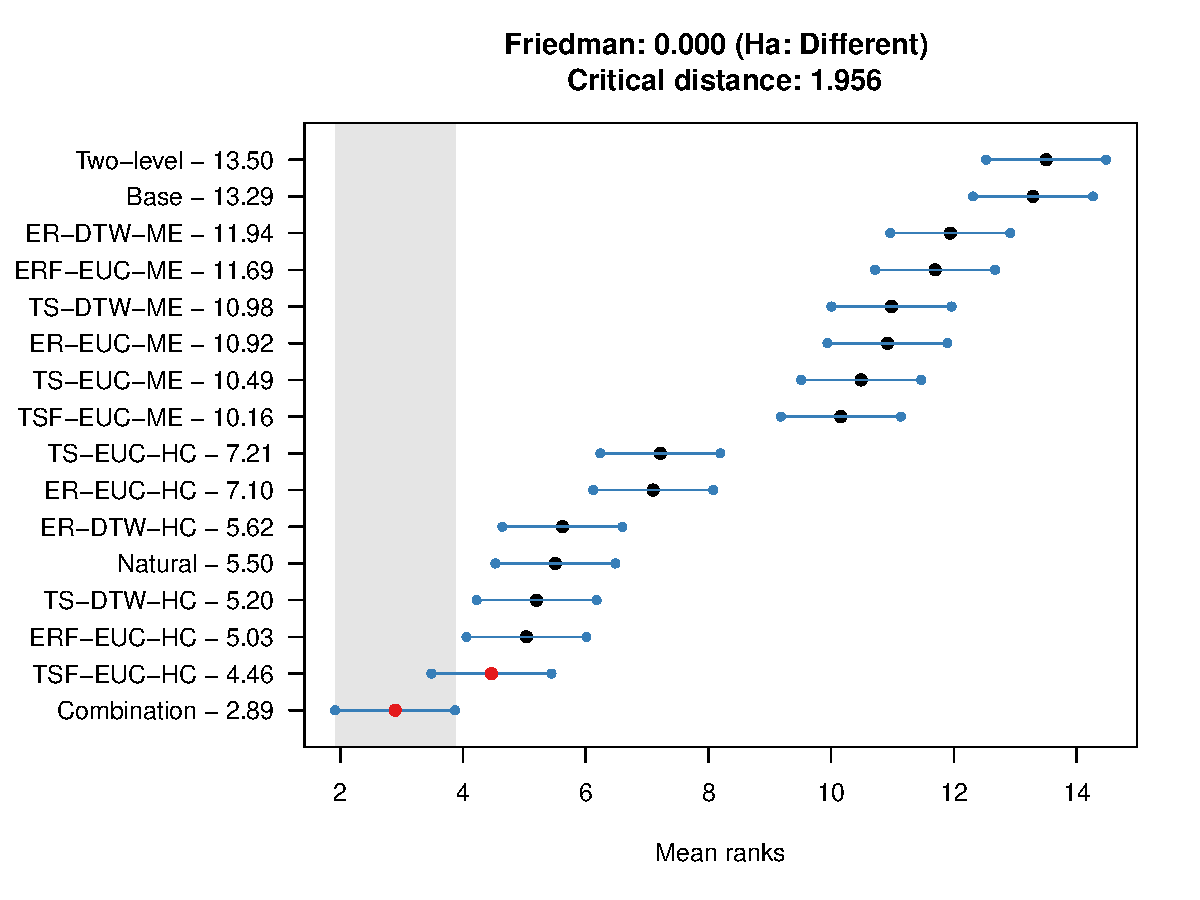
\includegraphics[width=0.45\textwidth]{figures/hierarchy_rmsse/tourism/P4_benchmarks_h12.pdf}
    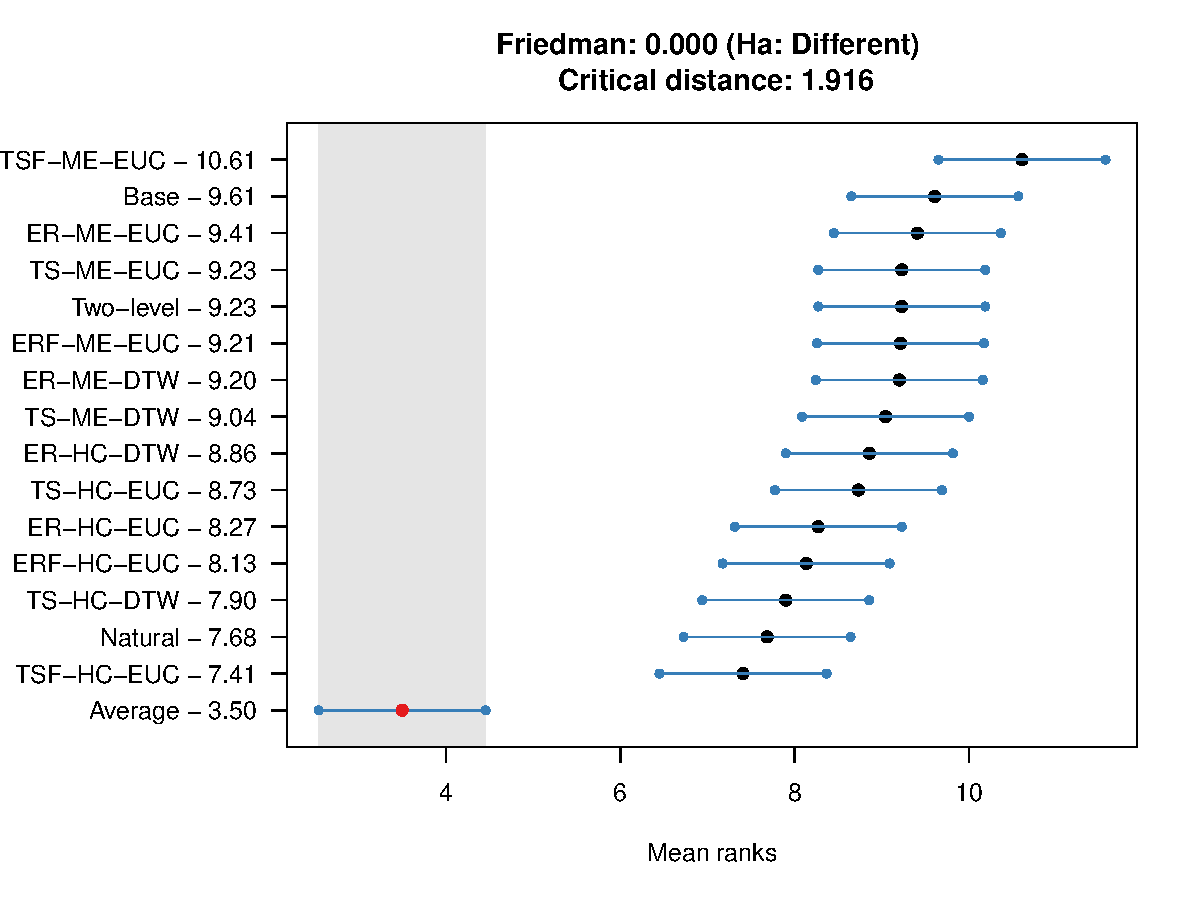
\includegraphics[width=0.45\textwidth]{figures/hierarchy_rmsse/mortality/P4_benchmarks_h12.pdf}
    \caption{Average ranks and 95\% confidence intervals for all approaches on tourism dataset(left) and mortality dataset(right) based on MCB test.}
    \label{fig:P4_bench_mcb}
\end{figure}


\subsection{Combination hierarchy vs its random twins}

We are also interested in if combination of cluster hierarchies significantly differ from its random twins. We propose to extend the permutation hierarchy generation approach introduced in Section~\ref{subsec:permutation} to combination hierarchy. 
First, we apply the same permutations of bottom-level series used in Section~\ref{subsec:P3_c_vs_pc} to all other cluster hierarchies.
Then for each of the $100$ permutations, the twelve reconciled forecasts obtained from corresponding random twins of cluster hierarchies are combined through equally-weighted combination, resulting $100$ random twins of combination hierarchy.
The results of MCB test for combination hierarchy and its $100$ random twins on the mortality dataset are presented in Figure~\ref{fig:P4_a_vs_pa}.
It is not surprising that the combination hierarchy ranks $100$th, given that even the best-performing cluster hierarchy failed to demonstrate absolute superiority.
This comparison is conducted solely on the mortality dataset, as computing random twins for all cluster hierarchies on the tourism dataset is time-consuming.
\begin{figure}[h!]
\vspace{-0.1in}
    \centering
    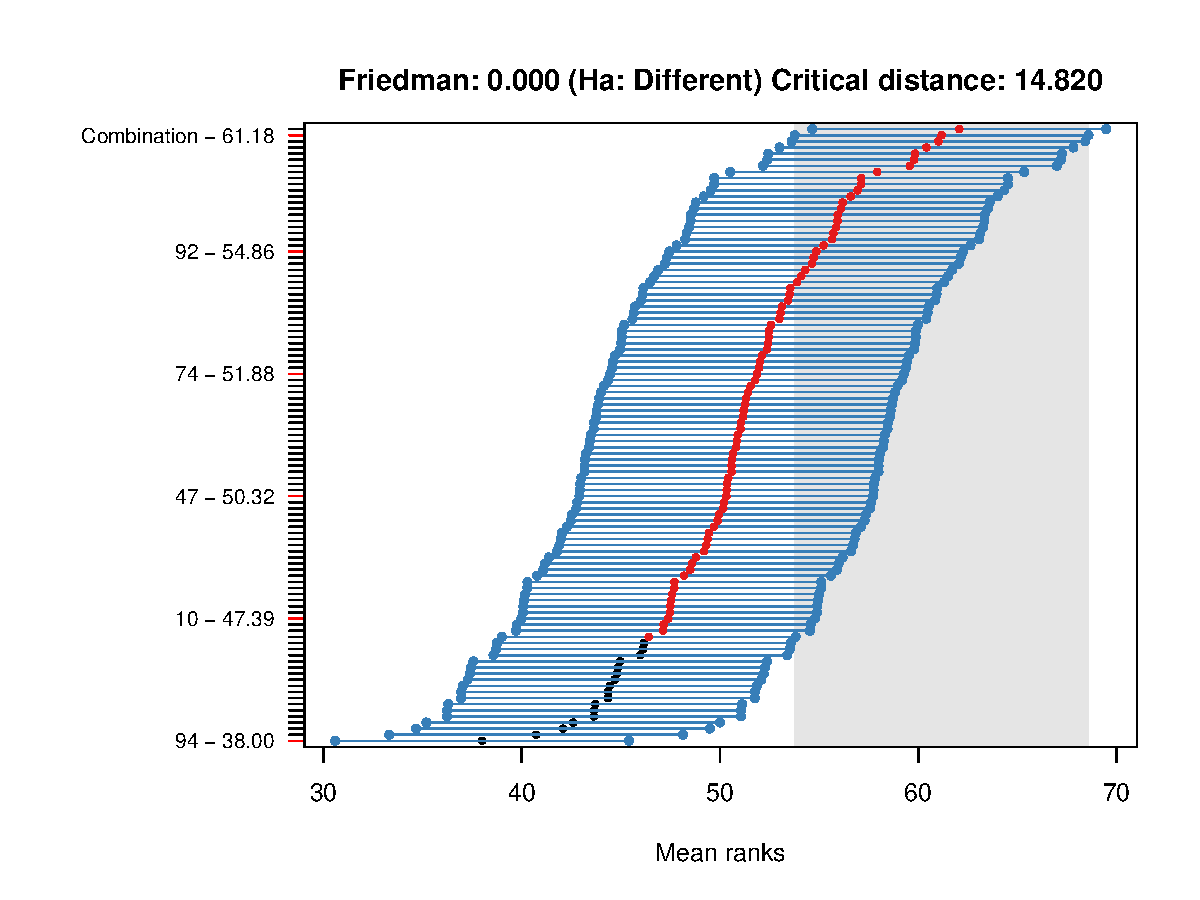
\includegraphics[width=0.75\textwidth]{figures/hierarchy_rmsse/mortality/P4_average_vs_pa_h12.pdf}
    \caption{\label{fig:P4_a_vs_pa} Average ranks and 95\% confidence intervals for combination of twelve cluster hierarchies and its $100$ random twins on mortality dataset based on MCB test.}
\end{figure}

\clearpage 
\newpage 

% \subsection{Results on simulation dataset}

% Table~\ref{}, Figures~\ref{} and We apply these analyses on the simulation dataset, leading to 


% \begin{figure}
%     \centering
%     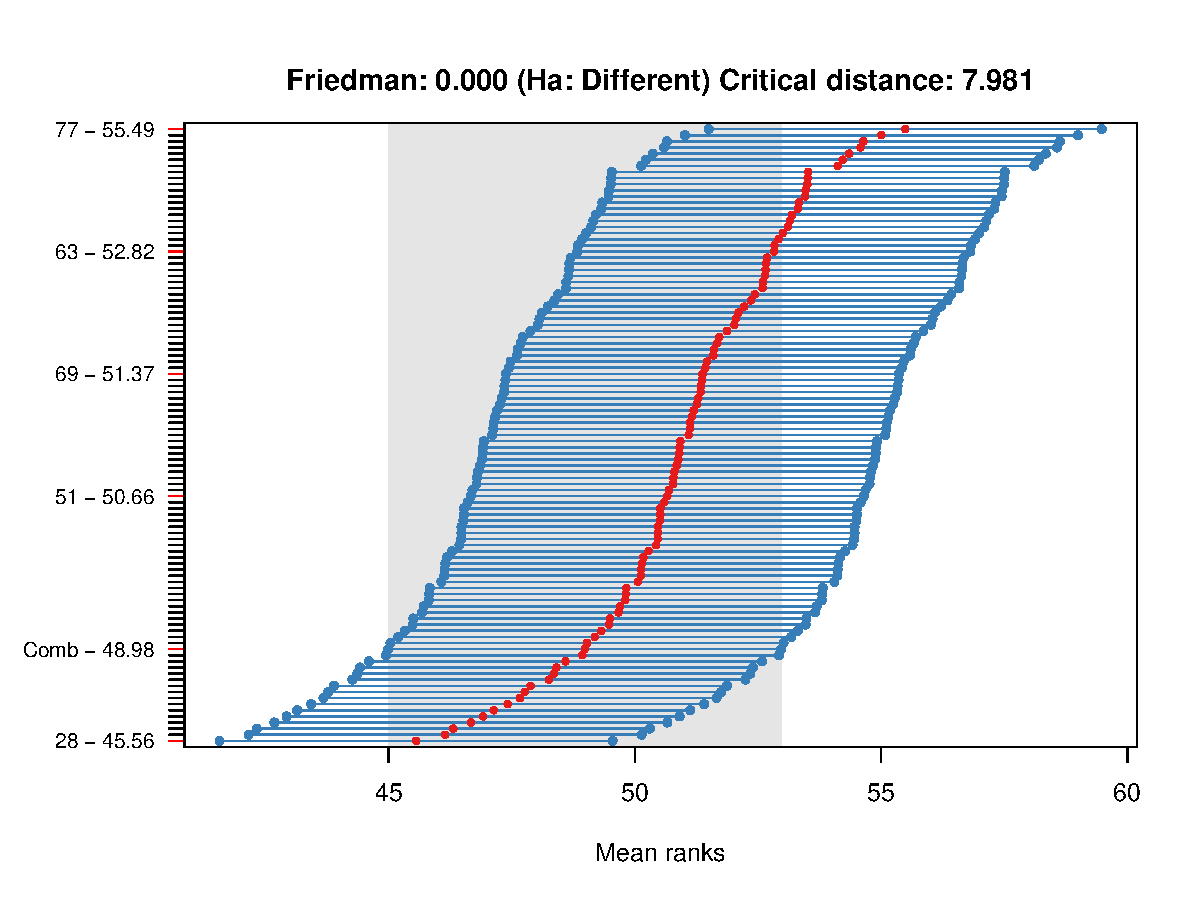
\includegraphics[width=0.8\textwidth]{figures/hierarchy_rmsse/simulation/P4.pdf}
%     \caption{}
%     \label{fig:}
% \end{figure}

\section{Discussion and Conclusion}
\label{sec:conclusion}

This paper extends the current body of research on clustering-based forecast reconciliation by introducing a general hierarchical forecasting framework, incorporating three distinct approaches: cluster hierarchies, random hierarchies, and combination hierarchies.
In contrast to the focused scope of previous studies, our approach to cluster hierarchies involves a broader exploration. We examine four time series representations, employ two distance measures, and utilize two clustering algorithms. This comprehensive method differs significantly from the existing literature, which typically concentrates on specific clustering implementations.
We also introduce two innovative random hierarchy construction methods to investigate what drives the performance enhancements in cluster hierarchies. These random hierarchies help isolate the effect of clustering, allowing us to focus on the benefits derived from the structure alone.
Furthermore, we propose combination hierarchies to mitigate uncertainties inherent in random hierarchies.

Our simulation study is constructed around two scenarios, each based on different base forecasting models. The first scenario highlights the value of the structure, evident in the high-ranking performance of random combination hierarchies. Structure can further improve forecast performance when the base forecasts are of high quality. The second scenario demonstrates the efficacy of clustering-based approaches, particularly when the base forecasts at the bottom level are less accurate.

Empirical studies on two datasets support our simulation findings. In the tourism dataset, the inferior base forecasts at the bottom level lead to all cluster hierarchies surpassing the original hierarchy, with four outperforming the combination of random hierarchies, which is used to demonstrate the impact of enriched structure. In contrast, the superior performance of two random combination hierarchies in the mortality dataset highlights the effectiveness of enriched structure. These results imply that the dominant factor, whether it is the enriched structure or clustering, varies depending on the dataset's characteristics, the base forecasting models, and other variables. Overall, our findings suggest that hierarchy construction approaches generally enhance performance, and combining these approaches leads to further improvements.


Future research based on our study could proceed in several promising directions. Firstly, our experiments were concentrated on total-level and bottom-level series. In practical applications, it might be necessary to include specific middle levels or evaluate the entire hierarchy. This could lead to the exploration of different hierarchy approaches, such as clustering middle-level series rather than bottom-level ones. Although we used equally-weighted combinations in this study, there's potential for applying more sophisticated methods to improve performance. The extensive literature on forecast combination, including advanced methods for calculating weights, offers numerous possibilities for enhancement (refer to \citealp{wangForecastCombinations50year2022} for an in-depth review).

% In Section~\ref{sec:combination}, we discuss the implications of combining multiple hierarchical structures on the uncertainty in estimating the covariance matrix of base forecast errors. Our conclusion was to opt for forecast combination rather than combining the structures of the hierarchies.  However, a systematic exploration of these two strategies, combining hierarchical structures and combining forecasts, presents an intriguing area for future research. Specifically, addressing the challenge of uncertainty due to high dimensionality in the combination of hierarchical structures is possible. In this context, innovative solutions like the regularized forecast reconciliation approach, as proposed by \cite{bentaiebRegularizedRegressionHierarchical2019a}, and alternative estimators of the covariance matrix, such as those suggested by \cite{pritulargaStochasticCoherencyForecast2021} could be highly beneficial. 

In both our simulation and empirical studies, the combination of random hierarchies displayed competitive results compared to clustering-based methods. However, the efficacy of this approach in scenarios with an extremely large number of bottom-level series remains uncertain. In such cases, a partially random approach might be more effective. For instance, initially generating random hierarchies, identifying those with superior performance, and then constructing partially random hierarchies based on these well-performing structures could be a viable strategy. Another intriguing possibility is the integration of both clustering and random approaches. Moreover, our study focused specifically on the aggregation of bottom-level series, which may have constrained the potential of middle-level series. It's plausible to enhance forecastability at the middle level by creating series through general linear combinations. 


Finally, our study was centered around point forecast reconciliation and cross-sectional hierarchy. However, the field of probabilistic forecast reconciliation has recently gained significant interest, as evidenced by research like \cite{panagiotelisProbabilisticForecastReconciliation2023} and \cite{jeonProbabilisticForecastReconciliation2019}. Applying hierarchy construction approaches to probabilistic forecast reconciliation presents a novel and potentially fruitful research avenue. This approach could provide deeper insights and more robust forecast reconciliation methods, particularly in scenarios where uncertainty and variability are significant factors.
Another promising direction for extending our methodologies lies in exploring temporal (\citealp{athanasopoulosForecastingTemporalHierarchies2017}) and cross-temporal hierarchies (\citealp{girolimettoCrosstemporalProbabilisticForecast2023a}). 


\clearpage 
\newpage 



%\section*{Acknowledgements}

%Bohan Zhang is supported by the international joint doctoral education fund of Beihang University.

\begingroup
\setstretch{1.15}
\bibliographystyle{agsm}
\bibliography{references.bib}
\endgroup



\end{document}